%===============================================================================
% LaTeX sjabloon voor de bachelorproef toegepaste informatica aan HOGENT
% Meer info op https://github.com/HoGentTIN/bachproef-latex-sjabloon
%===============================================================================

\documentclass{bachproef-tin}

\usepackage{hogent-thesis-titlepage} % Titelpagina conform aan HOGENT huisstijl
\usepackage[justification=centering]{caption}

%%---------- Documenteigenschappen ---------------------------------------------

% De titel van het rapport/bachelorproef
\title{Een vergelijkende studie van NLP-platformen voor
    het bouwen van een chatbot met een sterk
    begrijpend vermogen en lage foutenmarge}

% Je eigen naam
\author{Jarne Deschacht}

% De naam van je promotor (lector van de opleiding)
\promotor{Liesbeth Lewyllie}

% De naam van je co-promotor. Als je promotor ook je opdrachtgever is en je
% dus ook inhoudelijk begeleidt (en enkel dan!), mag je dit leeg laten.
\copromotor{Kenny Helsens}

% Indien je bachelorproef in opdracht van/in samenwerking met een bedrijf of
% externe organisatie geschreven is, geef je hier de naam. Zoniet laat je dit
% zoals het is.
%TODO KLOPT DIT ?
\instelling{In The Pocket}

% Academiejaar
\academiejaar{2019-2020}

% Examenperiode
%  - 1e semester = 1e examenperiode => 1
%  - 2e semester = 2e examenperiode => 2
%  - tweede zit  = 3e examenperiode => 3
\examenperiode{2}

%===============================================================================
% Inhoud document
%===============================================================================

\begin{document}

%---------- Taalselectie -------------------------------------------------------
% Als je je bachelorproef in het Engels schrijft, haal dan onderstaande regel
% uit commentaar. Let op: de tekst op de voorkaft blijft in het Nederlands, en
% dat is ook de bedoeling!

%\selectlanguage{english}

%---------- Titelblad ----------------------------------------------------------
\inserttitlepage

%---------- Samenvatting, voorwoord --------------------------------------------
\usechapterimagefalse
%%=============================================================================
%% Voorwoord
%%=============================================================================

\chapter*{\IfLanguageName{dutch}{Woord vooraf}{Preface}}
\label{ch:voorwoord}

%% TODO:
%% Het voorwoord is het enige deel van de bachelorproef waar je vanuit je
%% eigen standpunt (``ik-vorm'') mag schrijven. Je kan hier bv. motiveren
%% waarom jij het onderwerp wil bespreken.
%% Vergeet ook niet te bedanken wie je geholpen/gesteund/... heeft

Ik wil tijdens mijn professionele carrière met zoveel mogelijk technologieën in aanraking komen, omdat ik dat interessant vind. Hierdoor kan ik beter inschatten waar mijn grootste interesse ligt. Tijdens mijn opleiding heb ik nauwelijks inzicht gekregen in de wereld van artificiële intelligentie en machine learning en dat vond ik enorm jammer. Er was een opleidingsonderdeel in het derde jaar rond artificiële intelligentie, maar deze heb ik niet kunnen volgen doordat ik dat semester heb gekozen om te studeren in het buitenland. Tijdens deze periode heb ik dat vak op eigen initiatief bekeken en daar ontstond het idee om mijn bachelorproef te doen rond artificiële intelligentie, of toch een subdomein daarvan. De keuze om rond chatbots te werken kwam vrij snel, omdat ik altijd al geïnteresseerd was in hoe chatbots juist functioneren en hoe het kan dat een machine menselijke taal kan verstaan en zelf kan genereren. Het leek me leuk en leerrijk om dat zelf te kunnen bouwen. De bachelorproef leek me een ideaal moment om daar onderzoek rond te doen en mijn kennis daarin te verruimen.

Ik zou graag mijn promotor Liesbeth Lewyllie willen bedanken voor haar begeleiding en steun. Ze heeft me inhoudelijk en tijdens de uitwerking van dit onderzoek continu begeleid en telkens de nodige feedback voorzien. Bij vragen en onduidelijkheden over eender welk probleem kon ik bij haar terecht en heeft ze me steeds goed verder kunnen helpen.

Daarnaast wil ik ook mijn co-promotor Kenny Helsens bedanken om me vanaf het begin te ondersteunen in mijn idee. We hebben samen de scope van dit onderzoek vastgelegd en hij heeft me de vrijheid gegeven om een bachelorproef te maken waarin ik zelf veel beslissingen mocht maken. Zijn persoonlijke kennis en ervaring met het bedrijf In The Pocket hebben een duidelijke bijdrage geleverd in het eindresultaat.

Als laatste wil ik mijn vriendin Ime Van Daele bedanken om mijn bachelorproef meerdere malen te lezen en te verbeteren op grammaticale fouten. Alhoewel ze niet thuis is binnen dit onderzoekdomein, heeft ze dit werk met de nodige kritieke blik bekeken en nuttige feedback kunnen geven, wat zeker een positieve impact heeft.

%%=============================================================================
%% Samenvatting
%%=============================================================================

%  De "abstract" of samenvatting is een kernachtige (~ 1 blz. voor een
% thesis) synthese van het document.
%
% Deze aspecten moeten zeker aan bod komen:
% - Context: waarom is dit werk belangrijk?
% - Nood: waarom moest dit onderzocht worden?
% - Taak: wat heb je precies gedaan?
% - Object: wat staat in dit document geschreven?
% - Resultaat: wat was het resultaat?
% - Conclusie: wat is/zijn de belangrijkste conclusie(s)?
% - Perspectief: blijven er nog vragen open die in de toekomst nog kunnen
%    onderzocht worden? Wat is een mogelijk vervolg voor jouw onderzoek?
%
% LET OP! Een samenvatting is GEEN voorwoord!

%%---------- Nederlandse samenvatting -----------------------------------------
%
%  Als je je bachelorproef in het Engels schrijft, moet je eerst een
% Nederlandse samenvatting invoegen. Haal daarvoor onderstaande code uit
% commentaar.
% Wie zijn bachelorproef in het Nederlands schrijft, kan dit negeren, de inhoud
% wordt niet in het document ingevoegd.

\IfLanguageName{english}{%
\selectlanguage{dutch}
\chapter*{Samenvatting}
\lipsum[1-4]
\selectlanguage{english}
}{}

%%---------- Samenvatting -----------------------------------------------------
% De samenvatting in de hoofdtaal van het document

\chapter*{\IfLanguageName{dutch}{Samenvatting}{Abstract}}

Chatbots zijn tegenwoordig niet meer weg te denken uit onze maatschappij. We beseffen het niet altijd, maar we hebben meer interactie met een chatbot dan dat we initieel zouden verwachten. Denk hierbij bijvoorbeeld aan de klantenservice van bedrijven, want het gebeurt niet vaak meer dat ons eerste contact direct met een menselijke medewerker is als we bijvoorbeeld een chatbericht sturen naar de klantenservice van een bedrijf. Meestal is er een geautomatiseerde gesprekspartner geïmplementeerd om de klant verder te helpen bij problemen en vragen. Bedrijven gaan tegenwoordig vaak hun eigen chatbots bouwen, maar hoe moet dat juist? De ontwikkelingen binnen de wereld van artificiële intelligentie zijn de laatste jaren enorm sterk toegenomen. Deze ontwikkelingen bieden bedrijven de mogelijkheid om daarop in te spelen en er zelf mee te werken. Het implementeren van een chatbot vanaf het begin is een erg complex proces dat veel tijd en kennis vereist. Verschillende bedrijven hebben hierop ingespeeld door platformen te ontwikkelen die de implementatie van een chatbot vergemakkelijken. Hierdoor kunnen bedrijven, waar er onvoldoende kennis en tijd is voor de implementatie van chatbots, toch een chatbot bouwen en gebruiken. Er zijn tal van bedrijven die hun eigen chatbotplatformen hebben ontwikkeld waarmee eenvoudig een chatbot opgezet kan worden. Bedrijven zoals Google, Facebook, Microsoft, IBM, Amazon, etc. hebben allemaal zo’n platform gebouwd, maar welk van deze platformen is de beste?

Binnen deze bachelorproef is er een uitgebreid onderzoek gevoerd naar de verschillende gratis platformen die overweg kunnen met de Nederlandse taal, de meest interessante werden verder uitgediept. Daarbij werd er stilgestaan bij de verschillende functionaliteiten, de voor- en nadelen, de werking, de prestaties en de verschillende integratiemogelijkheden, zoals bijvoorbeeld met Slack of Facebook Messenger. De focus binnen deze bachelorproef ligt op het vinden van het platform die het best verstaat wat de gebruiker juist bedoeld en ook belangrijke informatie zoals datums, locaties, tijdstippen, etc. kan extraheren. Daarbij wordt ook rekening gehouden met spellingsfouten. De platformen zijn door middel van objectieve beoordelingstechnieken en verschillende experimenten getest. 

Het resultaat is dat het platform van Facebook (Wit.ai) algemeen de beste resultaten kan voorleggen. Zowel bij het correct verstaan van berichten als bij het afleiden van belangrijke informatie, scoort deze het sterkst. Het nadeel van Wit.ai is dat het moeite heeft met spellingsfouten en scoort daarbij minder goed in vergelijking met zijn concurrenten. IBM Watson kan hier de beste resultaten voorleggen. Ook de ingebouwde integratiemogelijkheden van andere platformen zijn geavanceerder dan die van Wit.ai, daarbij is Dialogflow de koploper met een grote verscheidenheid aan integraties.

Deze bachelorproef biedt veel mogelijkheden tot verder onderzoek, doordat de beoordeling werd beperkt tot de Nederlandse taal en doordat er geen betaalde platformen onderzocht werden. De dataset die werd gebruikt, is ook fictief en te klein om perfect representatief te zijn. Een onderzoek met een grotere representatieve dataset zou hier een oplossing voor kunnen bieden. Dit onderzoek is alvast een goed startpunt.































%---------- Inhoudstafel -------------------------------------------------------
\pagestyle{empty} % Geen hoofding
\tableofcontents  % Voeg de inhoudstafel toe
\cleardoublepage  % Zorg dat volgende hoofstuk op een oneven pagina begint
\pagestyle{fancy} % Zet hoofding opnieuw aan

%---------- Lijst figuren, afkortingen, ... ------------------------------------

% Indien gewenst kan je hier een lijst van figuren/tabellen opgeven. Geef in
% dat geval je figuren/tabellen altijd een korte beschrijving:
%
%  \caption[korte beschrijving]{uitgebreide beschrijving}
%
% De korte beschrijving wordt gebruikt voor deze lijst, de uitgebreide staat bij
% de figuur of tabel zelf.

\listoffigures
\listoftables

% Als je een lijst van afkortingen of termen wil toevoegen, dan hoort die
% hier thuis. Gebruik bijvoorbeeld de ``glossaries'' package.
% https://www.overleaf.com/learn/latex/Glossaries

%---------- Kern ---------------------------------------------------------------

% De eerste hoofdstukken van een bachelorproef zijn meestal een inleiding op
% het onderwerp, literatuurstudie en verantwoording methodologie.
% Aarzel niet om een meer beschrijvende titel aan deze hoofstukken te geven of
% om bijvoorbeeld de inleiding en/of stand van zaken over meerdere hoofdstukken
% te verspreiden!

%%=============================================================================
%% Inleiding
%%=============================================================================

\chapter{\IfLanguageName{dutch}{Inleiding}{Introduction}}
\label{ch:inleiding}

De inleiding moet de lezer net genoeg informatie verschaffen om het onderwerp te begrijpen en in te zien waarom de onderzoeksvraag de moeite waard is om te onderzoeken. In de inleiding ga je literatuurverwijzingen beperken, zodat de tekst vlot leesbaar blijft. Je kan de inleiding verder onderverdelen in secties als dit de tekst verduidelijkt. Zaken die aan bod kunnen komen in de inleiding~\autocite{Pollefliet2011}:

\begin{itemize}
  \item context, achtergrond
  \item afbakenen van het onderwerp
  \item verantwoording van het onderwerp, methodologie
  \item probleemstelling
  \item onderzoeksdoelstelling
  \item onderzoeksvraag
  \item \ldots
\end{itemize}

\section{\IfLanguageName{dutch}{Probleemstelling}{Problem Statement}}
\label{sec:probleemstelling}

Uit je probleemstelling moet duidelijk zijn dat je onderzoek een meerwaarde heeft voor een concrete doelgroep. De doelgroep moet goed gedefinieerd en afgelijnd zijn. Doelgroepen als ``bedrijven,'' ``KMO's,'' systeembeheerders, enz.~zijn nog te vaag. Als je een lijstje kan maken van de personen/organisaties die een meerwaarde zullen vinden in deze bachelorproef (dit is eigenlijk je steekproefkader), dan is dat een indicatie dat de doelgroep goed gedefinieerd is. Dit kan een enkel bedrijf zijn of zelfs één persoon (je co-promotor/opdrachtgever).

\section{\IfLanguageName{dutch}{Onderzoeksvraag}{Research question}}
\label{sec:onderzoeksvraag}

Wees zo concreet mogelijk bij het formuleren van je onderzoeksvraag. Een onderzoeksvraag is trouwens iets waar nog niemand op dit moment een antwoord heeft (voor zover je kan nagaan). Het opzoeken van bestaande informatie (bv. ``welke tools bestaan er voor deze toepassing?'') is dus geen onderzoeksvraag. Je kan de onderzoeksvraag verder specifiëren in deelvragen. Bv.~als je onderzoek gaat over performantiemetingen, dan 

\section{\IfLanguageName{dutch}{Onderzoeksdoelstelling}{Research objective}}
\label{sec:onderzoeksdoelstelling}

Wat is het beoogde resultaat van je bachelorproef? Wat zijn de criteria voor succes? Beschrijf die zo concreet mogelijk. Gaat het bv. om een proof-of-concept, een prototype, een verslag met aanbevelingen, een vergelijkende studie, enz.

\section{\IfLanguageName{dutch}{Opzet van deze bachelorproef}{Structure of this bachelor thesis}}
\label{sec:opzet-bachelorproef}

% Het is gebruikelijk aan het einde van de inleiding een overzicht te
% geven van de opbouw van de rest van de tekst. Deze sectie bevat al een aanzet
% die je kan aanvullen/aanpassen in functie van je eigen tekst.

De rest van deze bachelorproef is als volgt opgebouwd:

In Hoofdstuk~\ref{ch:stand-van-zaken} wordt een overzicht gegeven van de stand van zaken binnen het onderzoeksdomein, op basis van een literatuurstudie.

In Hoofdstuk~\ref{ch:methodologie} wordt de methodologie toegelicht en worden de gebruikte onderzoekstechnieken besproken om een antwoord te kunnen formuleren op de onderzoeksvragen.

% TODO: Vul hier aan voor je eigen hoofstukken, één of twee zinnen per hoofdstuk

In Hoofdstuk~\ref{ch:conclusie}, tenslotte, wordt de conclusie gegeven en een antwoord geformuleerd op de onderzoeksvragen. Daarbij wordt ook een aanzet gegeven voor toekomstig onderzoek binnen dit domein.
\chapter{\IfLanguageName{dutch}{Stand van zaken}{State of the art}}
\label{ch:stand-van-zaken}

In vorig hoofdstuk werd deze bachelorproef al kort ingeleid. In dit hoofdstuk zal de huidige kennis uit dit onderzoeksdomein verder besproken worden.

In sectie 2.1 zal er besproken worden wat chatbots zijn, welke soorten er bestaan, wat de voor-en nadelen zijn, wat de verbeterpunten en toekomstmogelijkheden zijn en hoe chatbots er voor staan op het vlak van beveiliging hoe dit verbeterd kan worden.

In sectie 2.2 wordt er ingezoomd op Natural Language Processing en de subdomeinen NLU en NLG.

In sectie 2.3 zullen de interessantste platformen kort geïntroduceerd worden en zullen ze vergeleken worden met elkaar op basis van een aantal basiscriteria. Binnen dit onderzoek worden geen volledig betalende/enterprise NLP-platformen vergeleken/toegelicht.

\newpage
\section{Chatbots}
\label{sec:chatbots}

\subsection{Soorten}
\label{subsec:soorten}

\subsubsection{Rule-based chatbot}
\label{subsubsec:chatbots-soorten-rule-based-chatbot}

Dit is de eenvoudigste en het traagste type chatbot. Deze bot bevat geen machine learning of artificiële intelligentie, maar werkt op basis van voorgeprogrammeerde regels. Bij dit type kan je enkel communiceren via een vaste selectie vragen/bevelen en kan je bij antwoord van de chatbot ook enkel terug antwoorden door uit een lijst te kiezen. Dit type zorgt voor weinig vrijheid, waardoor het ook enkel goed is voor basis klantvragen. Doordat alles manueel geprogrammeerd moet worden, is het ook telkens veel werk om nieuwe regels toe te voegen en de functionaliteit uit te breiden. Indien je een bericht stuurt naar deze bot die hij niet kent, dan weet hij ook gewoonweg niet wat hij ermee moet doen. Het voordeel van dit type is dan wel dat hij altijd accuraat antwoordt geeft, net doordat alles voorgedefinieerd is. Binnen deze bachelorproef zullen chatbots van dit type niet onderzocht en verder toegelicht worden.

\begin{figure}[!htbp]
    \label{fig:rule-based-chatbot-example}
    \centering
    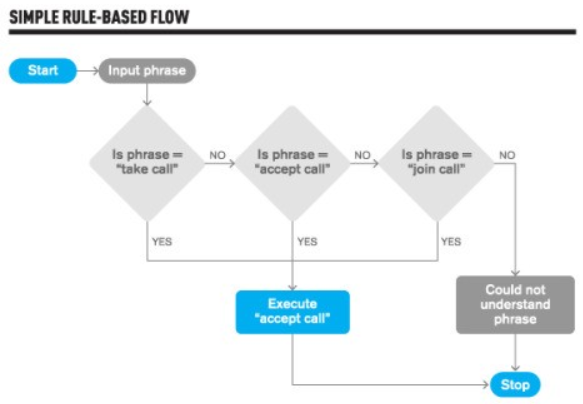
\includegraphics[width=0.8\textwidth]{rule-based-chatbot-example}
    \caption{Eenvoudige Flowchart van een rule-based chatbot \autocite{Shridhar2017}}
\end{figure}

\subsubsection{ML-based chatbot}
\label{subsubsec:chatbots-soorten-ml-based-chatbot}


Dit type chatbot wordt ook wel de NLP-chatbot of de AI-powered chatbot genoemd. Bij deze soort wordt in tegenstelling tot de rule-based chatbot wel sterk gebruik gemaakt van artificiële intelligentie en machine learning. De bot kan vragen beantwoorden die hij nog nooit eerder heeft gehoord en elimineert dus de limitatie van het rule-based type. NLP-chatbots leren van voorgaande taken en gaan op die manier zichzelf slimmer maken en hun kennis uitbreiden. Ze gebruiken ook speciale functies en algoritmes om de zinnen echt te verstaan en verder te verwerken. Dit type biedt de gebruiker veel meer vrijheid, maar is moeilijker om te ontwikkelen. De accuraatheid van deze soort is dan ook gemiddeld lager. Binnen deze bachelorproef zal de focus enkel liggen op chatbots van dit type. Wanneer er gesproken wordt over chatbots of gewoonweg bots, wordt er steeds een chatbot van dit type bedoeld.

\subsection{Voor-en nadelen}
\label{subsec:chatbots-voor-en-nadelen}

\subsubsection{Voordelen}
\label{subsubsec:chatbots-voor-en-nadelen-voordelen}

\begin{itemize}
    \item \textbf{Menselijke taken overnemen:} \\
    
    Chatbots worden ingezet voor heel wat verschillende toepassingen en kunnen menselijke taken overnemen. Een voorbeeld hiervan is reminders sturen van de agenda van een persoon zodat hij zelf niet meer hoeft te kijken. Chatbots nemen ook veel werk van de werknemers van klantendiensten en callcenters over door de grote hoeveelheid mensen die er kunnen geholpen en bereikt worden op hetzelfde moment. \\
    
    \item \textbf{Snellere interactie tussen onderneming en klant:} \\
    
    Uit een studie van \textcite{Social2016} blijkt dat klanten er van uit gaan dat er binnen de 4 uur een antwoordt wordt gegeven als er contact wordt opgenomen met de klantenservice via social media. Nu blijkt dat er in de realiteit een gemiddelde van 10 uur tussen zit voordat er een antwoordt wordt gegeven. Dit probleem wordt met chatbots onmiddellijk opgelost, omdat er real-time communicatie is tussen klant en bedrijf. Er wordt direct een antwoord gegeven en dat heeft een positieve invloed op de tevredenheid van klanten en het succes van ondernemingen. \\
    
    \item \textbf{Herkenbare interface:} \\
    
    Mensen zijn tegenwoordig volledig thuis binnen de verschillende messaging apps (Facebook, WhatsApp, Slack, …), omdat veel mensen het dag in dag uit gebruiken om te communiceren met vrienden, familie en collega’s. Chatbots bieden een conversatie interface aan die heel erg gelijklopend is met de interface waarmee mensen comfortabel zijn. Soms zijn ze zelfs volledige hetzelfde, bijvoorbeeld door een integratie met Facebook, WhatsApp of Slack. Doordat het herkenbaar overkomt, zullen geen mensen twijfelen om er gebruik van te maken. \\
    
    \item \textbf{Altijd beschikbaar:} \\
    
    Doordat chatbots geautomatiseerde gesprekspartners zijn, werken ze de hele dag door zonder vakanties te nemen en zonder ziek te vallen. Dit biedt voor gebruikers de mogelijkheid om eender wanneer op de dag gebruik te maken van deze systemen. \\
    
    \item \textbf{Kosten besparen:} \\
    
    Zonder een chatbot krijgt een bedrijf vaak dezelfde standaard vragen binnen van klanten. Om al deze vragen te beantwoorden zijn werknemers nodig en die moeten natuurlijk ook allemaal betaald worden en kunnen menselijke fouten maken. Door het implementeren van een bot, is er een aanzienlijke hoeveelheid werk die geautomatiseerd wordt, en dus geen menselijke acties meer vereisen. Op die manier kan een bedrijf besparen. \\
    
    \item \textbf{Data gebruiken voor verbeteringen:} \\
    
    Alle data die wordt verstuurd van en naar chatbots kunnen gemonitord en geanalyseerd worden. Daaruit kan worden afgeleid hoe de organisatie nog beter kan inspelen op de specifieke noden en eisen van het doelpubliek. \\ 
    
\end{itemize}

\subsubsection{Nadelen}
\label{subsubsec:chatbots-voor-en-nadelen-nadelen}

\begin{itemize}
    \item \textbf{Extra mogelijkheden voor cybercriminelen:} \\
    
    Mensen sturen regelmatig gevoelige informatie naar chatbots zoals kredietkaartgegevens, betalingsinformatie en wachtwoorden. Dit biedt cybercriminelen nieuwe mogelijkheden om deze informatie te onderscheppen en te misbruiken. Het is belangrijk hier de nodige aandacht aan te besteden. \\
    
    \item \textbf{Kan uit de hand lopen bij slechte supervisie:} \\
    
    Bots gaan leren van de informatie die ze krijgen toegestuurd om zichzelf slimmer te maken. Dit betekent dat het belangrijk is dat wij als mensen goed monitoren wat er allemaal gebeurt zodat niets uit de hand loopt. Een voorbeeld van slechte supervisie is de twitterbot Tay die in 2016 werd ontworpen door Microsoft als experiment. Mensen stuurden deze chatbot racistische informatie door en na minder dan een dag stuurde de bot zelf racistische tweets de wereld in. Kort daarna werd het experiment stopgezet \autocite{Vincent2016}. \\
    
\end{itemize}

\subsection{Verbetermogelijkheden}
\label{subsec:verbetermogelijkheden}

Volgens \textcite{Hussain2019} zijn er nog veel verbeterpunten mogelijk op het vlak van chatbots. Zo zou er meer focus moeten liggen op het beter verstaan van taalkundige elementen door bijvoorbeeld emotionele-en sentimentsanalyses uit te voeren. Chatbots zijn geen menselijke gesprekspartners en hebben dus ook geen emoties, maar emoties kunnen wel belangrijk zijn om een conversatie goed te laten verlopen. Tegenwoordig wordt hier sterk op ingezet, maar tot op heden staat dit nog niet op punt. Er zou ook een betere standaard moeten zijn om de kwaliteit van chatbots te testen.

Een eerder onderzoek heeft aangetoond dat mensen anders communiceren als ze weten dat ze met een machine converseren. Zo zouden mensen hun taal aanpassen als ze tegen een chatbot praten, zoals mensen ook doen als ze tegen een kind bezig zijn \autocite{Hill2015}. Het is uiteindelijk de bedoeling dat mensen niet weten ofdat ze tegen een chatbot praten of niet. Op die manier zullen ze hun taal niet aanpassen en zal het meest optimale resultaat behaald worden. 

Er zijn ook nog heel wat scenario’s waarbij chatbots geen gunstige antwoorden geven. Volgens \textcite{BRAIN2019} verstaan chatbots in 59\% van de gevallen regelmatig berichten niet zoals gehoopt en worden in 29\% van de gevallen accenten of taalvariaties niet goed verstaan. Er is dus zeker nog progressie nodig om het maximale uit chatbots te halen.

\subsection{Toekomstperspectief}
\label{subsec:toekomstperspectief}

Chatbots hebben nog veel groeimarge en zullen in de toekomst nog een stevigere marktpositie innemen. Volgens \textcite{Andreoli2017} is er een enorm potentieel voor conversationele banking. We komen in een tijdperk waarbij chatbots en messaging applicaties zoals Facebook Messenger, WhatsApp, … enorme populariteit verkrijgen, zelfs meer dan sociale media platformen. De banking industrie moet mee in dat tijdperk omdat chatbots bidirectionele interactie ondersteunen in real-time voor klanten, perfect geschikt zijn voor mobiele toestellen en zeer goed geïntegreerd kunnen worden in de verschillende messaging apps. 

Verder zullen chatbots volgens \textcite{Patel2020} ook op kwalitatief vlak sterk groeien in de toekomst. Zo zouden er betere sentimentsanalyses uitgevoerd worden om beter de emotie van klanten in te schatten en gepast te verwerken en te antwoorden. Chatbots zouden ook beter in staat zijn om dialecten en accenten goed op te vangen. Verder zullen ze in de komende jaren ook meer en meer deel worden van ons dagelijkse leven.  

Chatbots zouden zich in de toekomst ook meer en meer gaan gedragen als mensen en daarbij zal het onderscheiden van bots en echte gesprekspartners moeilijker worden. Tegenwoordig gedragen bots zich nog vaak oppervlakkig en hebben ze geen persoonlijkheid en komen onnatuurlijk over. Facebook is op dit moment sterk aan het inzetten op het geven van een echte persoonlijkheid aan hun chatbots. Daarbij zouden chatbots zich meer gedragen als een echt persoon met specifieke karaktereigenschappen \autocite{Carey-Simos2018}.

\subsection{Security}
\label{subsec:security}

Chatbots beloven veel voordelen, maar er is ook redelijk wat speculatie rond de veiligheid van deze systemen. Chatbots bieden voor cybercriminelen nieuwe manieren om data te onderscheppen van gebruikers. Veel data die circuleert tussen mens en bot zijn niet gevoelig, maar soms kunnen kredietkaartgegevens, logingegevens en dergelijke wel passeren. Deze data mag natuurlijk niet onderschept worden, want dat zou problemen veroorzaken als dat in de verkeerde handen komt. Organisaties maken zich zorgen over hoe veilig chatbots zijn, waar informatie opgeslagen wordt en hoe alles beveiligd wordt \autocite{Shanbhag2018}.


volgens \textcite{Shanbhag2018} zijn er een aantal manieren om de beveiliging van chatbots te verbeteren:

\begin{itemize}
    \item \textbf{End-to-end encryptie:} \\
    
    Data die verstuurd wordt is volledig versleuteld waardoor het niet leesbaar is voor eventuele mensen die het onderscheppen. Enkel zender en ontvanger kunnen het lezen. \\
    
    \item \textbf{Two-factor authenticatie:} \\
    
    Identiteit van chatbot gebruikers moet bevestigd worden door twee verschillende kanalen. Voorbeelden van deze kanalen zijn webpagina’s, sms’en, vingerafdruk, etc. \\
    
    \item \textbf{Authenticatie timeouts:} \\
    
    Gebruikers worden automatisch uitgelogd als ze een bepaalde tijd inactief zijn. \\
    
    \item \textbf{Biometrische authenticatie:} \\
    
    Identiteit bevestigen door vingerafdruk en gezichtsherkenning. \\
    
    \item \textbf{Self-destructing messages:} \\
    
    Gevoelige data die wordt verstuurd over het kanaal wordt na een bepaalde tijd voor eeuwig vernietigd. \\
\end{itemize}

Een aantal van deze technieken worden in de meeste chatbots automatisch toegepast.


\section{Natural Language Processing (NLP)}
\label{sec:nlp}

\subsection{Natural Language Understanding (NLU)}
\label{subsec:nlp-nlu}

Natural Language Understanding is een onderdeel van NLP en is een techniek die verantwoordelijk is om aan de hand van algoritmes, machines te leren om menselijke taal (tekst of spraak) te verstaan en te interpreteren. NLU gebruikt vele technieken zoals sentiments-en-contextuele analyses en gaat ook de relatie tussen woorden in zinnen achterhalen. Ook slecht gevormde zinnen en woorden moeten verstaan worden. Het doel van NLU is om de intentie van de berichten te achterhalen. Daarbij is NLU ook verantwoordelijk om de juiste parameters/entities te achterhalen. Intenties kunnen op veel verschillende manieren geformuleerd worden. Bijvoorbeeld, de zin “welk weer is het buiten” kan je op honderden manieren formuleren, maar de intentie/de bedoeling is steeds hetzelfde, te weten komen welk weer het is buiten.


\subsection{Natural Language Generation (NLG)}
\label{subsec:nlp-nlg}


Natural Language Generation is ander onderdeel van NLP en is een techniek waarbij structurele data (input) wordt omgezet in natural language, dat is menselijke taal. Menselijke tekst of spraak wordt dus gegenereerd door machines. In deze bachelorproef zal er niet verder worden ingegaan op NLG, maar zal de focus enkel liggen op het begrijpend vermogen van de chatbots (NLU).


\subsection{NLP vs NLU}
\label{subsec:nlp-nlp-vs-nlu}


De termen NLP en NLU worden vaak met elkaar verward en door elkaar gebruikt. NLU is een onderdeel van NLP en bij het verstaan van menselijke tekst, gaat NLP kijken naar wat er is gezegd terwijl NLU gaat kijken wat er is bedoeld. NLP kan tekst en spraak analyseren, verschillende technieken toepassen met bedoeling om menselijke input (ongestructureerde data) om te zetten in structurele data, maar de bedoeling/intentie van berichten achterhalen is een specifieke taak van NLU. 

\begin{figure}[!htbp]
    \label{fig:nlp-nlu-nlg}
    \centering
    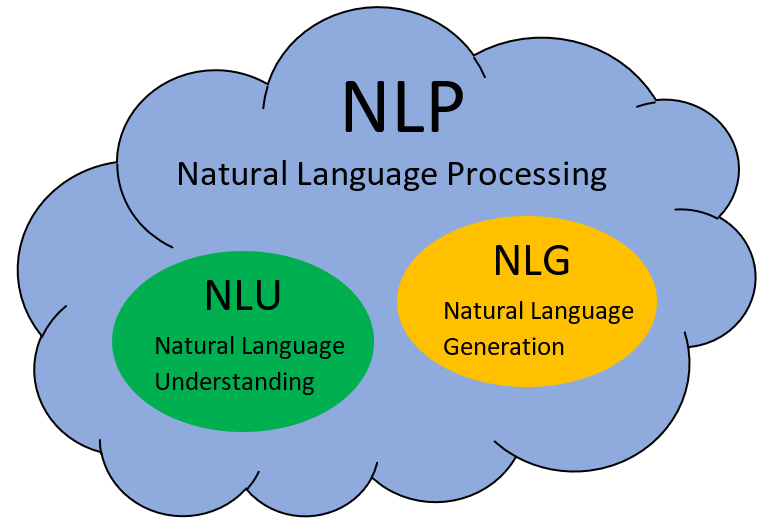
\includegraphics[width=0.5\textwidth]{nlp-nlu-nlg}
    \caption{Grafische voorstelling van NLP en de subdomeinen NLU en NLG \autocite{Sciforce2019}}
\end{figure}

\section{NLP-platformen}
\label{sec:nlp-platformen}

Er zijn tientallen platformen op de markt waarmee chatbots kunnen gebouwd worden. De grootste en meest consistente zijn ontwikkeld en onderhouden door de grote marktspelers zoals Google, Microsoft, IBM, Facebook en Amazon. Een van de zaken die gebouwd kunnen worden met al deze platformen is bijvoorbeeld een chatbot. Ze bieden een gebruiksvriendelijke interface aan waarmee heel eenvoudig chatbots kunnen ontwikkeld worden. Ze hebben ook allemaal hosting mogelijkheden en ingebouwde integraties waarmee zonder moeite de gebouwde bots op andere platformen zoals apps, websites, social media, etc. kunnen gebruikt worden. Binnen vele studies worden hun platformen vaak naar voor geschoven in vergelijking met de kleinere. Daarom zal de vergelijkende studie zich dan ook vooral focussen op platformen die door hen zijn aangeboden omdat zij het kapitaal en de mogelijkheden hebben om te blijven innoveren en hun platformen verder te ontwikkelen. Er zal 1 platform worden onderzocht die nogal sterk afwijkt van de andere. Dat is omdat dit platform vaak sterk concurreert binnen vergelijkende studies met de andere traditionele. Er zullen enkel platformen worden bekeken die ondersteuning bieden voor de nederlandse taal, omdat dit een absolute vereiste is voor klanten van In The Pocket die op de belgische markt actief zijn. Het platform van Amazon zal niet worden opgenomen, omdat hun tool geen Nederlands ondersteund. Verder zullen ook geen betalende platformen worden opgenomen, omdat er voor deze bachelorproef daar geen budget voor is.

\subsection{Dialogflow}
\label{subsec:nlp-platformen-dialogflow}

Dialogflow (vroeger API.ai) is een mens-computer interactie service waarmee verschillende zaken ontwikkeld kunnen worden op basis van natuurlijke taal (Natural Language). Het platform is grotendeels gratis, maar de enterprise edities bieden nog uitgebreidere functies aan. Het is ontwikkeld en onderhouden door Google en maakt gebruik van de infrastructuur en ML-algoritmes van Google. Dialogflow is onderdeel van het Google Cloud Platform (GCP), dat is een platform die heel wat diensten aanbiedt voor applicatie infrastructuur, gegevensbeheer, analyses, machine learning en artificiële intelligentie, beveiliging, etc. Dialogflow is ook geoptimaliseerd voor het gebruik van Google Assistant. Er is ook ondersteuning voorzien voor meer dan 20 talen en er zijn veel intents en entities voorzien die je als ontwikkelaar zomaar out-of-the-box kan gebruiken. Er zijn ook al voorgebouwde chatbots aanwezig voor vaak voorkomende scenario’s die je zomaar kunt gebruiken. Dit platform kan ook geïntegreerd worden in heel erg veel andere diensten. Grote bedrijven zoals Domino’s Pizza, Mercedes, Comcast, Ticketmaster en Giorgio Armani maken onder andere gebruik van Dialogflow voor hun chatbots \autocite{Dialogflow2020}. 

\subsection{IBM Watson}
\label{subsec:nlp-platformen-ibm-watson}

IBM Watson is het NLP-platform van IBM en is net zoals Dialogflow geschikt voor het bouwen van chatbots. Dit platform is deel van IBM cloud, waardoor veel diensten van daar kunnen gebruikt worden. Watson kan voor een beperkt aantal conversaties gratis worden gebruikt. Watson is gebouwd op neurale netwerken, waardoor het heel erg goed kan leren van vorige conversaties. Het ondersteund 13 talen en ook ingebouwde entities. Er zijn ook verschillende integratiemogelijkheden voorzien. IBM Watson staat ook gekend als een platform die heel erg gebruiksvriendelijk is en waarmee in weinig tijd een chatbot kan opgezet worden. Met klanten als The North Face en Chevrolet moeten ze dus zeker niet onderdoen voor de concurrenten \autocite{IBM2020}.


\subsection{LUIS}
\label{subsec:nlp-platformen-luis} 

LUIS is de NLU tool aangeboden door Microsoft en is ook een vaste waarde op de markt. Met LUIS op zich kan geen volledige chatbot worden gebouwd, omdat het enkel NLU diensten aanbiedt en dus enkel dient voor intent classificatie en niet voor het antwoorden naar eindgebruikers toe.  Het kan daarentegen wel makkelijk geïntegreerd worden met het Microsoft Bot Framework, waarin wel de logica zit om complexe dialogen te voeren. LUIS is ook onderdeel van Microsoft Azure, waardoor het ook met deze cloud functies goed kan samenwerken. LUIS maakt gebruik van een speciale active learning technologie waardoor het beter overweg zou kunnen met nieuwe trainingsdata. Er zijn 13 talen ondersteund en ook opnieuw vele ingebouwde intents en entities \autocite{LUIS2020}.

\subsection{Wit.ai}
\label{subsec:nlp-platformen-wit.ai}

Wit.ai is een open-source platform die ontwikkeld is door Facebook. Het is volledig gratis en ondersteund bijna alle talen die er bestaan. Het is een platform door en voor ontwikkelaars en doordat het open source is, is elke interactie gedeeld met de volledige community. Doordat het ontwikkeld is door Facebook, heeft het wel een beperkt aantal integraties (enkel websites, apps en Facebook Messenger) \autocite{Wit2020}.

\subsection{RASA}
\label{subsec:nlp-platformen-rasa}

Het laatste platform die onderzocht wordt is eentje die nogal sterk afwijkt van de andere. Het is verschillend, omdat het ten eerste niet wordt aangeboden door een groot bedrijf zoals Google, Facebook of Microsoft, maar ook omdat het volledig open-source is. Het is ook geen platform die zoals de rest bereikt kan worden via het internet met een user interface. Dit framework moet gedownload worden en dan kan er lokaal een chatbot worden gebouwd. Indien dit platform bereikbaar moet zijn vanop het internet, dan moet de ontwikkelaar daar zelf voor instaan. Het kan wel mits wat configuratie op Google Cloud, Microsoft Azure of Amazon Web Services (AWS) gezet worden. Deze tool vereist heel wat meer technische kennis van ontwikkelaars, maar biedt wel meer mogelijkheden om een chatbot te bouwen die aangepast is aan de noden van een project. Rasa bestaat uit rasa NLU en rasa core.  Rasa NLU staat in voor het classificeren van de intents en het verstaan van berichten en rasa core is een engine om dialogen te voeren. Binnen dit onderzoek zal enkel rasa NLU gebruikt worden. Doordat rasa open-source, kan er als ontwikkelaar zelf worden gekozen welke componenten worden gebruikt. Dit zorgt er voor dat het vrijwel mogelijk is om in elke taal een chatbot met rasa te bouwen. Er zijn ook heel wat componenten beschikbaar om gebruik te maken van voorgemaakte entities en intents. Rasa wijkt sterk af van de andere platformen, maar is zeker interessant om te onderzoeken, omdat het ook vaak in voorgaande studies sterk uit de hoek kwam en omdat het heel sterk op maat geïmplementeerd kan worden \autocite{RASA2020}.

\subsection{Vergelijking van platformen}
\label{subsec:nlp-platformen-vegelijking-platformen}

%TODO tabel hier in toevoegen

De platformen die hierboven besproken werden, werden ook al vaak in voorgaande studies met elkaar vergeleken. Daaruit bleken telkens andere platformen de bovenhand te nemen. Deze onderzoeken werden ook niet in het Nederlands gedaan, dus een nederlandse vergelijking anno 2020 is dan ook zeker niet overbodig.

Volgens het onderzoek van \textcite{Russis2018} is de tool die IBM aanbiedt om chatbots in de cloud te bouwen veruit de beste op de markt met als dichtste achtervolgers Microsoft (LUIS) en Google (Dialogflow). Dit wordt dan weer betwist door het onderzoek van \textcite{Langen2017}, want zij besluiten dat LUIS (Microsoft) veruit het beste platform is. De eerstvolgende achtervolger is RASA. de resultaten van RASA kwamen vrij dicht in de buurt van die van LUIS. Het grote voordeel van RASA is dat het door de ontwikkelaar helemaal zelf geconfigureerd kan worden, waardoor het beter aangepast kan worden aan een specifieke use case. Het zou dus zeker kunnen dat RASA beter kon presteren dan LUIS mits iets meer configuratie op maat. Dit maakt RASA interessant om verder te onderzoeken.

Volgens het onderzoek van \textcite{Savenkov2017} Is ook IBM Watson de winnaar op het vlak van intent classificatie. Daarnaast zijn Api.ai (nu Dialogflow) en LUIS de eerstvolgende achtervolgers. De verschillen van prestaties tussen die drie zijn relatief klein.

Een ander onderzoek geeft dan weer aan dat Snips.ai de beste NLU heeft met als eerstvolgende achtervolgers Wit.ai en Dialogflow. Snips.ai op zich is een platform die ook interessante mogelijkheden biedt om verder te onderzoeken, maar dit platform ondersteund geen Nederlands en is dus niet relevant voor dit onderzoek. Interessant is wel dat Wit.ai en Dialogflow de eerstvolgende achtervolgers zijn \autocite{Coucke2017}.

Uit de verschillende onderzoeken hierboven beschreven kwamen bijna altijd andere platformen naar boven met de beste prestaties voor intent classificatie. Er moet ook rekening gehouden worden met het feit dat deze onderzoeken al enige tijd geleden zijn uitgevoerd en dat de platformen en technologieën binnen AI en ML continu blijven evolueren en dus nu al sterk veranderd zullen zijn. Deze bachelorproef zal een oplossing bieden voor deze onduidelijkheden door een onderzoek anno 2020 uit te voeren.

















%%=============================================================================
%% Methodologie
%%=============================================================================

\chapter{\IfLanguageName{dutch}{Methodologie}{Methodology}}
\label{ch:methodologie}

In dit hoofdstuk zal er een experiment worden toegelicht die op een objectieve manier het begrijpend vermogen van de platformen zal beoordelen.

In sectie \ref{sec:opzet} staan we stil bij de opzet van het experiment en hoe de platformen geëvalueerd zijn.

In sectie \ref{sec:dataset} voorzien we meer uitleg rond het testscenario en de opgestelde dataset.

In sectie \ref{sec:validatie} wordt er toegelicht hoe de platformen op een objectieve manier geëvalueerd en vergeleken worden.

In sectie \ref{sec:werking-platformen} illustreren we de werking en functionaliteiten van de verschillende platformen. Daarbij wordt stilgestaan bij het creëren van een chatbot, het toevoegen van verschillende intents, het trainen met voorbeeldzinnen en hoe de gebouwde chatbots getest kunnen worden. 

In sectie \ref{sec:automatisatie} zal ten slotte meer informatie worden gegeven rond de praktische implementatie van het experiment en hoe het trainen en testen van de platformen geautomatiseerd wordt.


\section{Opzet}
\label{sec:opzet}

Om een vergelijking te kunnen maken van het begrijpend vermogen van de platformen, moet er een experiment plaatsvinden waarbij er op een objectieve manier beoordeeld wordt. Daarom werd er een dataset opgesteld waarmee alle platformen zullen getraind en geëvalueerd worden. Op deze manier krijgen alle platformen exact dezelfde informatie en kan er objectief beoordeeld worden. Een deel van de dataset zal gebruikt worden voor het trainen van de chatbots en het andere deel zal dienen voor het testen. Deze dataset zal bestaan uit een aantal intents met bijbehorende voorbeeldzinnen die bij dat bepaalde intent horen. Op deze manier kunnen de machine learning algoritmes modellen bouwen, die de juiste intent herkennen als een gebruiker een bericht naar de chatbot stuurt. Indien intents geen voorbeeldzinnen krijgen, dan zal het trainen onmogelijk zijn, wat een sterke invloed zal hebben op de accuraatheid. De meeste platformen vereisen een minimum van vijf voorbeeldzinnen om het trainen te kunnen starten, maar het is sterk aangewezen om minimum 10-15 voorbeeldzinnen per intent te voorzien \autocite{Greyling2019}. Eens het trainen gedaan is, kan het valideren beginnen. Het is de bedoeling om uiteindelijk een platform aan te duiden die het beste begrijpend vermogen heeft en dus het beste presteert op het herkennen van de juiste intent. Er zal op drie verschillende manieren geëvalueerd worden. Het hoofddoel van dit onderzoek is om te bepalen welk platform het beste presteert op intentherkenning. Daarbij wordt er beoordeeld op de prestaties bij zowel het gebruik met, als het gebruik zonder entities. Het is algemeen aangeraden om entities te gebruiken, maar in dit onderzoek wordt er ook gekeken naar de invloed op de resultaten als er entities worden gebruikt in tegenstelling tot de resultaten waar de entities zijn weggelaten. Daarnaast wordt er ook beoordeeld hoe goed de getrainde applicaties om kunnen gaan met taalvariaties. Gebruikers schrijven regelmatig geen standaard Nederlands als ze communiceren via het internet, daarom wordt er verwacht dat ze dit ook niet zullen doen als ze praten met een chatbot. Daardoor is het belangrijk dat een chatbot ook de intentie van berichten kan verstaan als gebruikers afkortingen, dialecten en slecht gevormde woorden en zinnen gebruiken.

\section{Dataset}
\label{sec:dataset}

De dataset is opgesteld op basis van een fictieve use case die werd bepaald in samenwerking met de co-promotor. Het is de bedoeling om een virtuele assistent te bouwen voor een busreisorganisatie. Het bedrijf wil mee met de digitale evolutie en wil gebruikers de mogelijkheid geven om interactie aan te gaan met een geautomatiseerde gesprekspartner om informatie te krijgen, eventuele klachten af te handelen en busreizen te boeken en te beheren. Daarbij zijn er een aantal intents gedefinieerd.

Er werd gekozen voor de volgende intents:
\begin{itemize}
    \item begroetingen
    \item geefBestemmingen
    \item geefReisTijden
    \item boekBusreis
    \item geefActueleInfo
    \item wijzigBusreis
    \item annuleerBusreis
    \item geefOnboardServices
    \item meldKlachten
    \item huurBusMetChauffeur
\end{itemize}

Voor het valideren van entityherkenning werd gekozen voor de volgende entities:
\begin{itemize}
    \item locatie
    \item datum
    \item aantal\_tickets
    \item tijdstip
    \item onboardService\_type
\end{itemize}

De entity onboardService\_type is een zelfgemaakte entity. Voor de andere entities werd gebruik gemaakt van systeementities die ingebouwd zitten in het platform. Op deze manier kunnen we de prestaties van zowel systeementities als zelfgemaakte entities beoordelen.


Elk van de intents werd voorzien van vijftien voorbeeldzinnen. Bij het opstellen van de voorbeeldzinnen was het belangrijk dat er rekening werd gehouden met een aantal zaken \autocite{Greyling2019}:
\begin{itemize}
    \item Gebruik korte en lange zinnen
    \item Verschillende synoniemen gebruiken
    \item Varieer de positie van entities
    \item Wissel grammatica af
    \item Gebruik woorden zowel in enkelvoud als in meervoud
    \item Gebruik niet altijd hoofdletters en leestekens
\end{itemize}

\section{Validatie}
\label{sec:validatie}

Chatbots zijn voorbeelden van gesuperviseerd leren, daarbij is het de bedoeling dat er op basis van trainingsdata modellen worden opgesteld die voor ongekende input de correcte output kunnen voorspellen. Dit zal ook binnen dit experiment worden toegepast. Er zijn vijftien voorbeeldzinnen voorzien per intent en het is de bedoeling dat er een deel van deze zinnen worden gebruikt om de chatbots te trainen. Het resterende deel wordt gebruikt om te valideren dat het model de juiste intent kan herkennen bij een gegeven input.

De meest gebruikte methode is om 80\% van de data te gebruiken om te trainen en dat de resterende 20\% wordt gebruikt om te testen \autocite{Desmarais2018}. Deze methode is vrij eenvoudig te implementeren, maar het probleem hierbij is dat niet alle data voor zowel trainen als testen gebruikt wordt. Dat kan resulteren in minder accurate resultaten.

De oplossing voor dit probleem is K-Fold Cross Validation \autocite{Desmarais2018}. Hierbij wordt de dataset in een aantal gelijke delen verdeeld en wordt er één deel gebruikt voor het testen, waarbij de resterende delen worden gebruikt om te trainen. Dit wordt een aantal keer herhaald, afhankelijk van het aantal delen dat je hebt gekozen, dat zijn het aantal cycli die doorlopen worden. Het meest gebruikte aantal delen is vijf, omdat er op deze manier aan het 80/20 principe kan voldaan worden. Vier delen worden dan gebruikt om de chatbot te trainen (80\%) en het andere deel om te valideren (20\%). Bij een volgende cyclus wordt er dan doorgeschoven. Het grote voordeel van deze methode is dat het veel betrouwbaarder en robuuster is, omdat er vijf keer zoveel testen zijn in vergelijking met de andere methode. Hierbij wordt ook alle data gebruikt voor zowel het trainen als het testen, wat het probleem van de bovenstaande methode oplost.

\begin{figure}[H]
    \label{fig:cross-validation-schema}
    \centering
    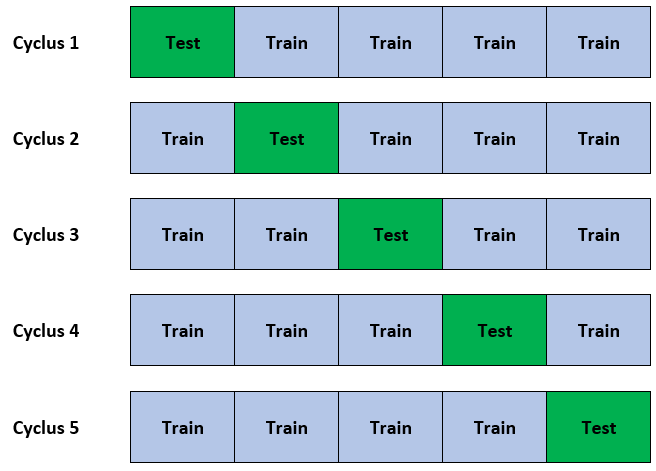
\includegraphics[width=0.85\textwidth]{schema-cross-validation}
    \caption{Grafische voorstelling van de werking van cross validation}
\end{figure}

\subsection{Confusion matrix}
\label{subsec:validatie-confusion-matrix}

Een confusion matrix is een duidelijke representatie van de resultaten van een classificatieprobleem. Het is een overzicht van hoeveel keer een categorie voorspeld werd en hoeveel keer dit juist of fout was. Het is ook duidelijk zichtbaar welke categorie werd gekozen indien het niet correct is. Vanuit een confusion matrix kunnen  interessante metrieken berekend worden. Berekeningen kunnen worden gedaan per categorie of in het geheel. Een voorbeeld van een confusion matrix voor een classificatieprobleem wordt geïllustreerd in onderstaande afbeelding. In dit onderzoek wordt vaak gebruik gemaakt van confusion matrices om de resultaten per platform te berekenen.

\begin{figure}[H]
    \label{fig:confusion-matrix-voorbeeld}
    \centering
    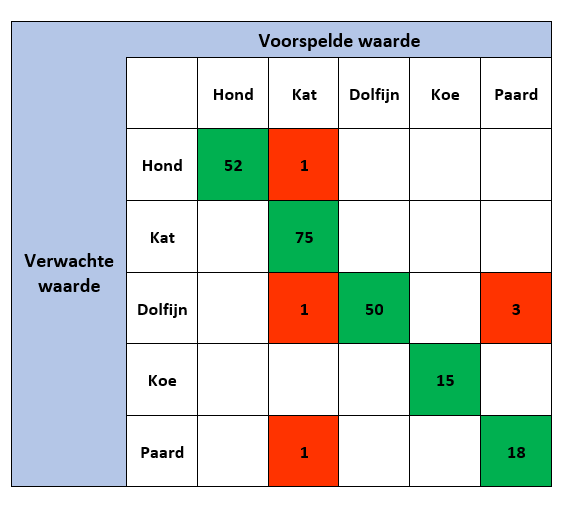
\includegraphics[width=0.85\textwidth]{confusion-matrix-voorbeeld}
    \caption{Voorbeeld van een confusion matrix}
\end{figure}

De linkerkant (de rijen) staan voor het dier die verwacht wordt en de kolommen staan voor het dier die voorspeld is. Hieruit kunnen er een aantal conclusies genomen worden:
\begin{itemize}
    \item Er zijn 53 (52+1) gevallen waarbij een hond verwacht werd. In 52 gevallen werd dit ook effectief voorspeld door het model. Eén keer werd een fout dier voorspeld, namelijk een kat.
    \item De katten en de koeien werden altijd voorspeld als ze verwacht werden.
    \item De dieren hond, dolfijn en koe werden nooit voorspeld als ze niet verwacht werden.
\end{itemize}

\subsection{Precision, Recall \& F-score}
\label{subsec:validatie-precision-recall-f-score}

Er zijn een aantal interessante metrieken die berekend kunnen worden uit een confusion matrix. Deze metrieken worden gebruikt om platformen met elkaar te vergelijken. Deze metrieken kunnen zowel berekend worden per intent/categorie, als in het geheel.

\subsubsection{Precision}

Precision is een metriek die aangeeft in hoeveel procent van de gevallen de voorspelde waarde ook effectief de juiste blijkt te zijn.
In bovenstaand voorbeeld kan er worden afgeleid dat een paard 21 (18+3) keer werd voorspeld. In 18 gevallen blijkt dit ook correct te zijn. Dat betekend dat de precision van deze categorie ongeveer 86\% (18/21) is. 

\subsubsection{Recall}

Recall is een andere metriek die aangeeft hoeveel procent van de categorieën correct voorspeld zijn. In bovenstaand voorbeeld zijn er 19 (18+1) voorbeelden waarbij een paard verwacht werd. In 18 gevallen werd het juiste dier herkend. Dat betekent dat de recall voor deze categorie ongeveer 95\% (18/19) is.

Initieel lijken de metrieken precision en recall sterk op elkaar, maar toch zijn ze volledig verschillend van elkaar, dat bewijst het voorbeeld.

\subsubsection{F-score}

Precision en recall vertellen weinig over de kwaliteit van het model \autocite{Treml2019}. Ze zijn enkel nuttig indien je zowel de precision als de recall kent. Om dit samen te voegen in één duidelijke metriek, bestaat er de F-score. Dat is het harmonisch gemiddelde van de recall en de precision. De F-score vertelt hoe kwalitatief een classificatiemodel is. Hoe hoger de F-score, hoe beter. Binnen dit onderzoek wordt de F-score gebruikt om de resultaten van de verschillende platformen met elkaar te vergelijken.

De F-score (harmonisch gemiddelde) bereken je als volgt:
\begin{itemize}
    \item F-score $= 2 * \frac{precision*recall}{precision+recall}\\$
\end{itemize}

In het voorbeeld van het paard is de F-score ongeveer gelijk aan 90\%.


\section{Werking van de platformen}
\label{sec:werking-platformen}


In deze sectie zal worden toegelicht hoe de verschillende platformen functioneren, dit is een belangrijk onderdeel binnen dit onderzoek. Er zal stilgestaan worden bij het creëren van een chatbot, het toevoegen van intents, het trainen met voorbeeldzinnen en hoe de gebouwde chatbots getest kunnen worden. Binnen deze sectie zullen ook de verschillende functionaliteiten van platformen worden toegelicht die niet gebruikt zijn voor het experiment. Dit experiment focust zich op het classificeren van intents en niet op een volledige conversatie met de chatbot. Toch is het belangrijk om stil te staan bij de mogelijkheden van elk platform om een volledig beeld te krijgen.

\subsection{Dialogflow}
\label{subsec:werking-platformen-dialogflow}

Dialogflow is een gebruiksvriendelijk platform dat zowel voor technische als geen technische mensen bruikbaar is, het helpt wel als je enige technische kennis hebt om alles beter te verstaan. Het enige dat nodig is om aan de slag te gaan met Dialogflow is een Google account. Iedereen kan ermee aan de slag, omdat het grotendeels gratis is. De betaalde versie is eerder voor bedrijven die complexe chatbots willen creëren die gebruik maken van functies die niet in de gratis versie zitten zoals de sentimentanalyses. De betalende versie is ook handig voor bedrijven die chatbots willen opzetten die meer verzoeken per minuut kunnen behandelen dan de limiet voor de gratis versie (zie sectie \ref{subsec:nlp-platformen-vegelijking-platformen}). Doordat Dialogflow onderdeel is van het Google Cloud Platform, kan er ook eenvoudig gebruik worden gemaakt van de diverse services van Google. Er zijn vele analysemogelijkheden aanwezig die gebruikt kunnen worden om de prestaties te monitoren. Dialogflow gebruikt de term agenten (agents) voor hun chatbots, ze doen dit, omdat ze de vergelijking willen maken met menselijke callcenter agenten \autocite{GoogleCloud2020}. Agenten verwerken conversaties met eindgebruikers, er zijn heel wat voorgebouwde agenten beschikbaar die gratis gebruikt kunnen worden. Bij het maken van een agent moet een naam opgegeven worden en moet er een standaardtaal gekozen worden. Het is mogelijk om extra talen toe te voegen indien er een meertalige agent gebouwd moet worden. Het is ook mogelijk om de agent te linken aan een Google Cloud project, op die manier is de samenwerking met andere diensten eenvoudiger. 

\begin{figure}[H]
    \label{fig:dialogflow-create}
    \centering
    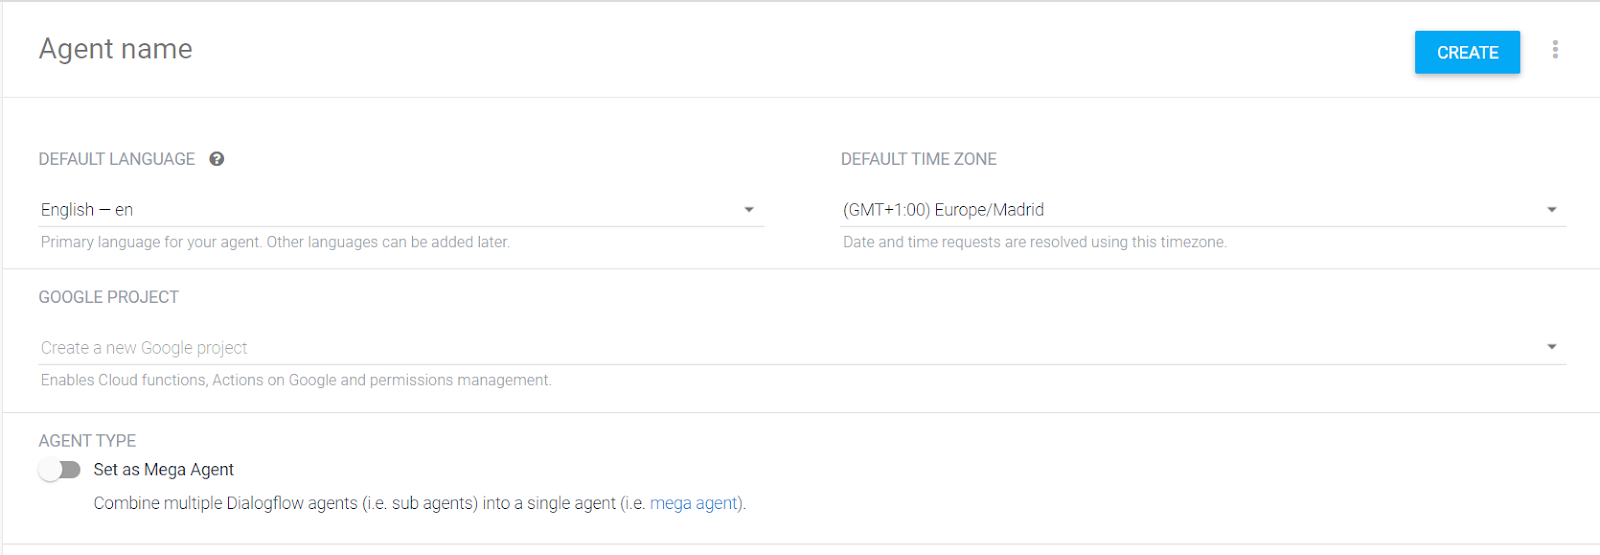
\includegraphics[width=\textwidth]{dialogflow-create}
    \caption{Het creëren van een agent in Dialogflow}
\end{figure}

Agenten gebruiken intents om de intentie van berichten die gebruikers sturen te achterhalen. Bij het toevoegen en configureren van de intents, moet er een naam opgegeven worden en kunnen er diverse trainingszinnen toegevoegd worden. Dialogflow vereist een minimum van vijf voorbeeldzinnen per intent. Het is ook mogelijk om in de voorbeeldzinnen entities/parameters toe te voegen, er zijn heel wat entities ingebouwd in het systeem die gratis gebruikt kunnen worden. Per intent kunnen er ook antwoorden voorzien worden die de agent stuurt als die intent geclassificeerd wordt.

\begin{figure}[H]
    \label{fig:dialogflow-intent}
    \centering
    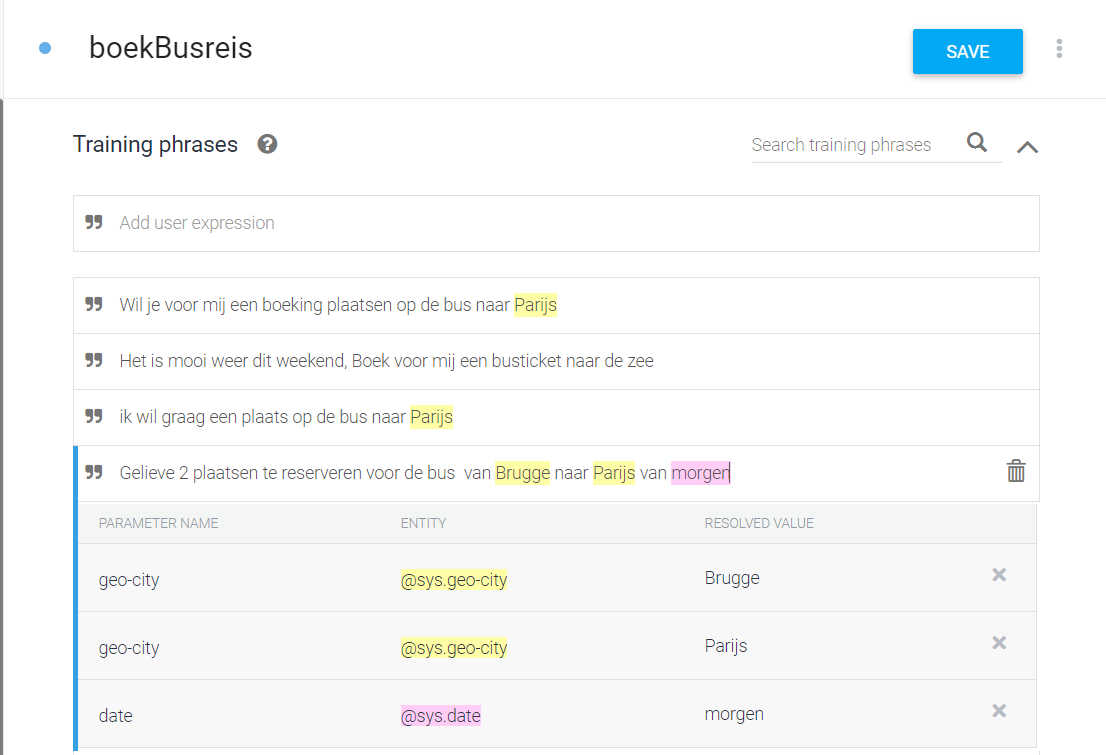
\includegraphics[width=\textwidth]{dialogflow-intent}
    \caption{Het aanmaken van een intent met voorbeeldzinnen in Dialogflow waarbij er ook entities worden aangeduid}
\end{figure}

In Dialogflow is het mogelijk om contexten te gebruiken, dit is gelijkaardig met de context in natuurlijke taal. Indien iemand zegt `Ik koop het`, dan moet de chatbot weten waar die 'het' naar verwijst. Dialogflow maakt gebruik van input en output contexten en kunnen toegevoegd worden aan intents. Input contexten zijn parameters die doorgegeven moeten worden aan een specifieke intent, voordat de die uitgevoerd kan worden. Output contexten zijn parameterwaarden die herkend worden in de intent en actief worden, zodat ze dan als input contexten in andere intents gebruikt kunnen worden. Bij elke intput context die er wordt toegevoegd, wordt er automatisch ook een output context toegevoegd. Het is wel mogelijk om extra output contexten toe te voegen indien dit nodig is. Onderstaande afbeelding bevat een voorbeeld van hoe contexten gebruikt kunnen worden in Dialogflow. Om de intent 'AnnuleerBusreis' uit te voeren, is het vereist dat de bestemming en datum gekend zijn, zonder die informatie is het niet mogelijk om te weten wat juist geannuleerd moet worden. Contexten en entities lijken erg op elkaar en dit kan voor verwarring zorgen. Een context is niets meer dan een entity die globaal gebruikt en doorgegeven kan worden doorheen verschillende intents. Contexten zullen in deze bachelorproef niet worden gebruikt, maar het is wel een interessante functie die Dialogflow heeft.

\begin{figure}[H]
    \label{fig:dialogflow-context}
    \centering
    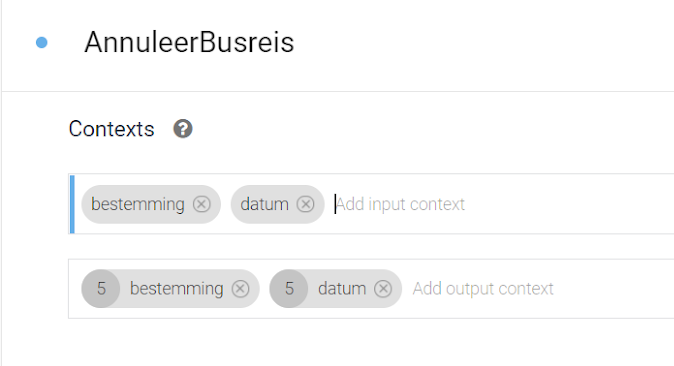
\includegraphics[width=0.7\textwidth]{dialogflow-context}
    \caption{Het toevoegen van contexten in een intent in Dialogflow}
\end{figure}

Aangezien er heel wat systeementiteiten zijn voorzien in Dialogflow, kan het zijn dat het niet meteen nodig is om zelf entities aan te maken, maar het is wel mogelijk. Bij het aanmaken van een entiteit kunnen verschillende waarden toegevoegd worden om de agent deze entiteit te doen herkennen bij user input. Er kunnen synoniemen gegeven worden en er is een mogelijkheid om een specifiek patroon op te geven waarvoor een entiteit herkend wordt in zinnen. De gemaakte entiteiten kunnen dan net zoals systeementiteiten toegevoegd worden aan voorbeeldzinnen in de intents. In deze bachelorproef wordt indien mogelijk altijd 'fuzzy matching' gebruikt bij de entiteiten. Deze optie zorgt ervoor dat woorden die verkeerd geschreven zijn en spellingsfouten bevatten, toch herkend kunnen worden als entiteit zonder dat de woorden perfect juist geschreven hoeven te zijn.

\begin{figure}[H]
    \label{fig:dialogflow-entity}
    \centering
    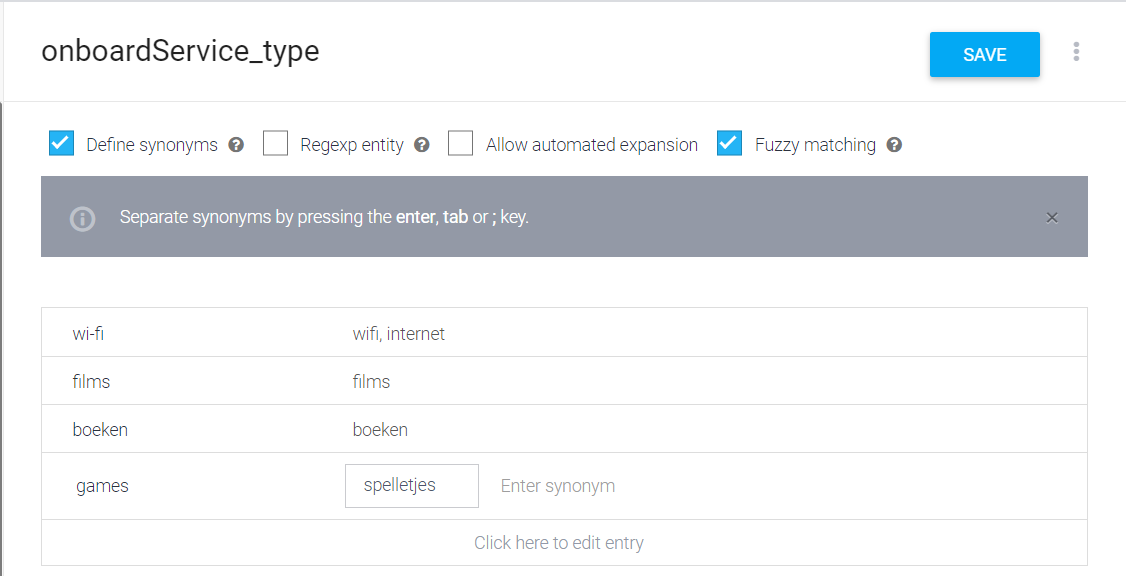
\includegraphics[width=\textwidth]{dialogflow-entity}
    \caption{Het aanmaken en beheren van een entiteit in Dialogflow}
\end{figure}

Met Dialogflow is het mogelijk om als ontwikkelaar eerdere berichten die eindgebruikers hebben gestuurd naar de agent te valideren, zodat die zinnen gebruikt kunnen worden als extra voorbeeldzinnen bij de intents. Op deze manier wordt de agent steeds slimmer doorheen zijn levensloop, doordat hij meer data krijgt. In onderstaande afbeelding is weergegeven hoe je dit als ontwikkelaar kunt doen. Alle berichten die gebruikers naar de agent hebben gestuurd, staan hier chronologisch weergegeven. Daarbij staat ook vermeld welke intent herkend werd door de agent op dat moment. Door middel van de vinkjes, annuleer-tekens of vuilbakjes, kun je aangeven wat je hiermee precies wilt doen. Met een groen vinkje bevestig je dat de herkende intent ook de juiste was en met het vuilbakje geef je aan dat het fout was en dat je dit niet wil toevoegen als een extra voorbeeldzin. De annuleer-tekens worden gebruikt om aan te geven dat de intentherkenning fout was en dat je dit bericht wilt toevoegen aan de default fallback intent. Indien een intentherkenning fout was, kun je ook de herkende intent wijzigen en toch goedkeuren. Met de approve knop bovenaan, wordt alles definitief opgeslaan en verdwijnen deze berichten uit de lijst. De berichten waarbij er een groen vinkje stond, worden toegevoegd als nieuwe voorbeeldzinnen bij de respectievelijke intent. Op termijn kun je op deze manier een erg grote lijst van voorbeeldzinnen per intent bekomen, wat goed is voor de kwaliteit van de agent.

\begin{figure}[H]
    \label{fig:dialogflow-validate}
    \centering
    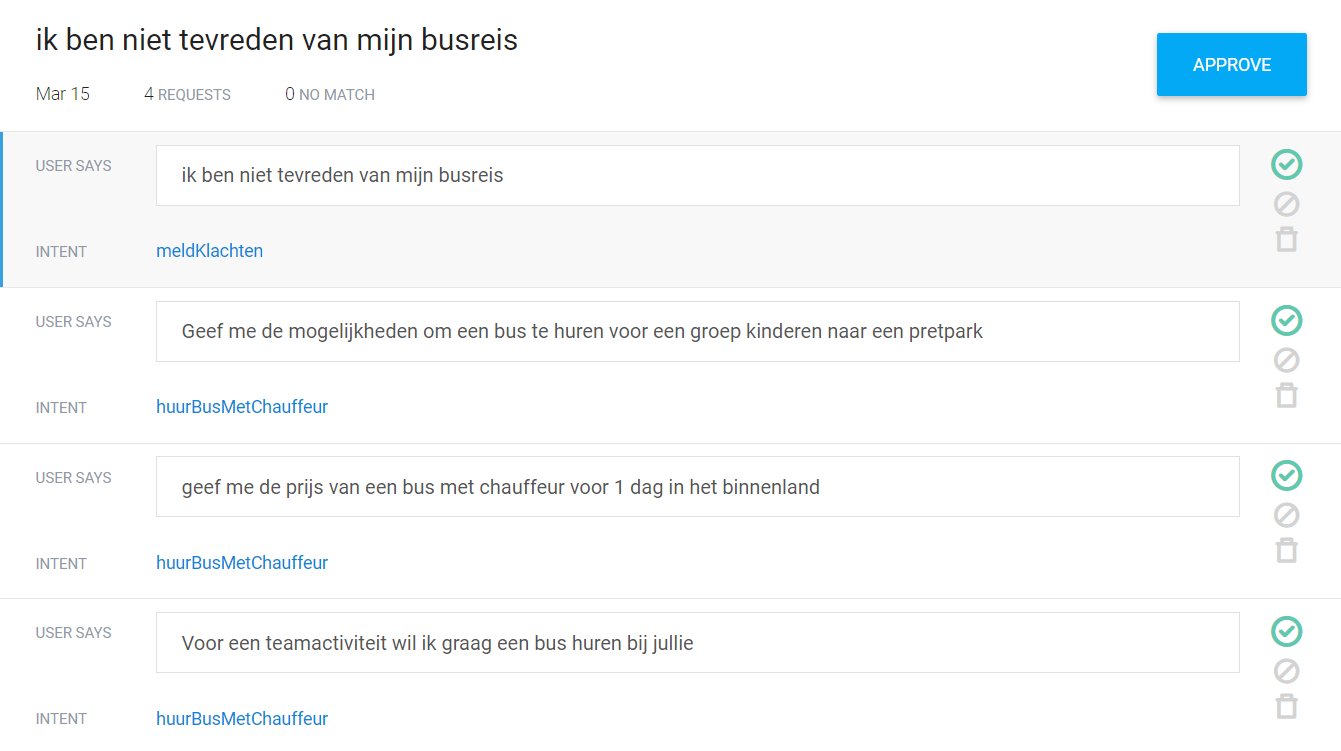
\includegraphics[width=\textwidth]{dialogflow-validate}
    \caption{Het valideren van user input om het model uit te breiden in Dialogflow}
\end{figure}

Dialogflow is eenvoudig te integreren met andere diensten. Het enige dat je hiervoor als ontwikkelaar moet doen, is de integratie aanzetten op een scherm in Dialogflow. Er komt daarna informatie beschikbaar op het scherm die uitlegt wat je precies moet doen om het werkende te krijgen. Het is ook mogelijk om zelf een applicatie te schrijven die gebruik maakt van de API van Dialogflow.

\begin{figure}[H]
    \label{fig:dialogflow-integrations}
    \centering
    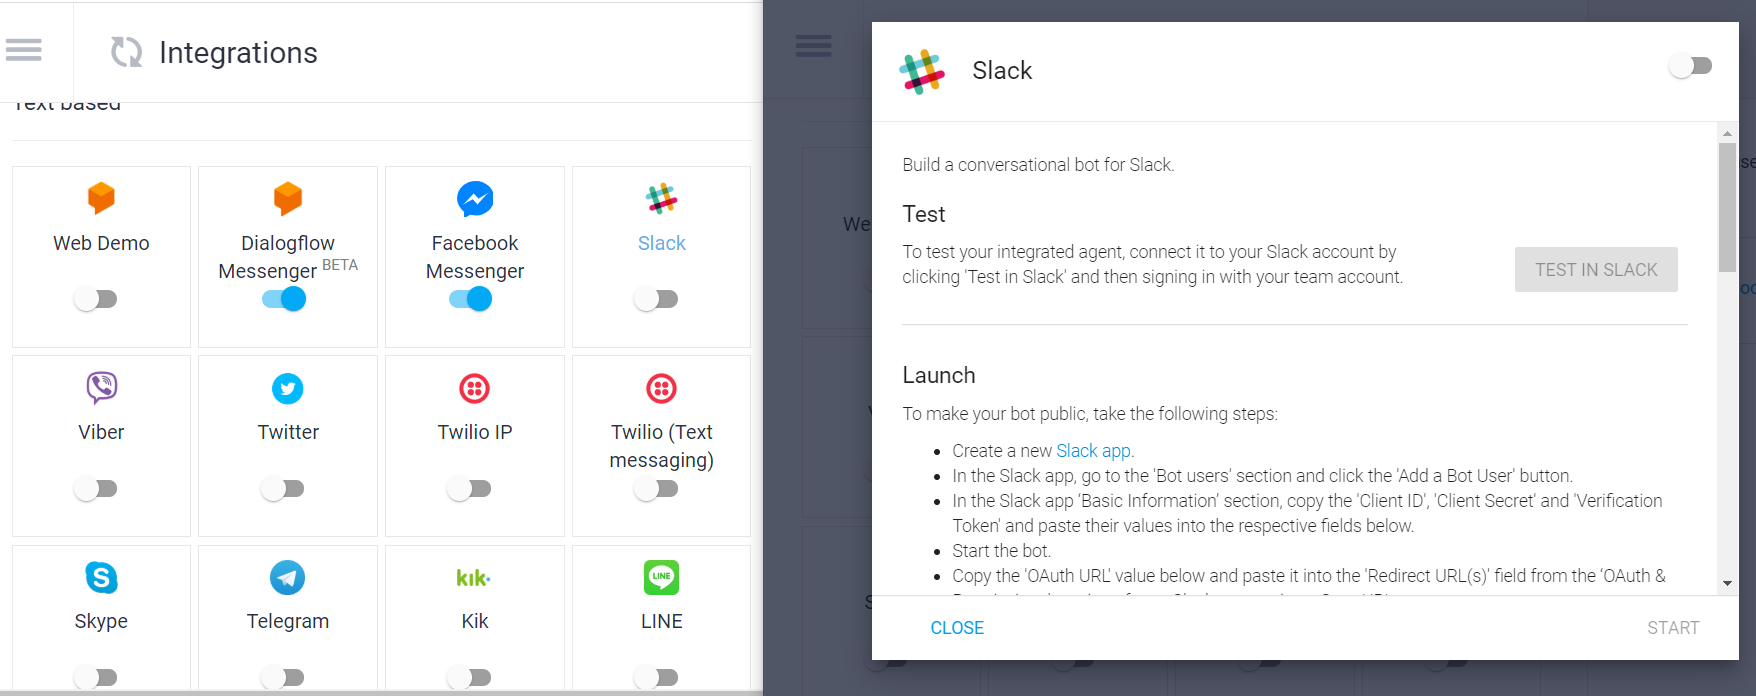
\includegraphics[width=\textwidth]{dialogflow-integrations}
    \caption{Het integreren van een Dialogflow agent in andere diensten}
\end{figure}

De chatbot testen kan via de user interface (UI) gebeuren. Dit kan worden gedaan door een bericht te sturen naar de ingebouwde conversatiemodule. Bij het sturen van een bericht krijg je informatie over welke intent is herkend, wat het antwoord is en welke paramaters herkend werden. Het is ook mogelijk om meer gedetailleerde resultaten te zien. Opnieuw zal er in deze bachelorproef geen speciale aandacht besteed worden aan het antwoorden naar gebruikers.

\begin{figure}[H]
    \label{fig:dialogflow-test}
    \centering
    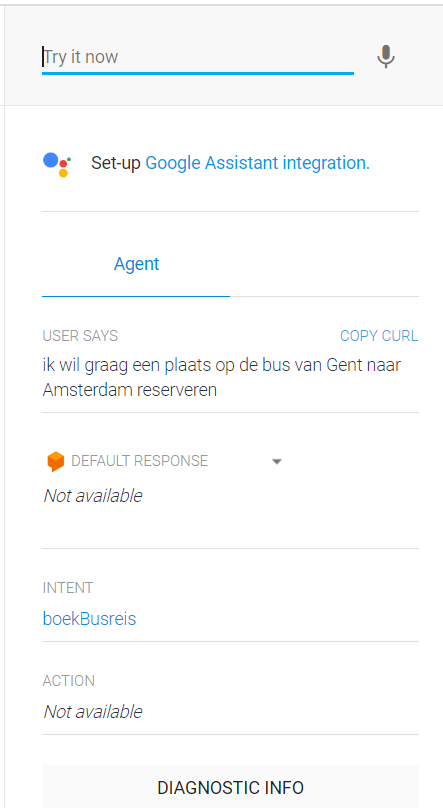
\includegraphics[width=0.5\textwidth]{dialogflow-test}
    \caption{Het testen van de agent met de conversatiemodule in Dialogflow}
\end{figure}

\subsection{IBM Watson}
\label{subsec:werking-platformen-ibm-watson}

IBM Watson is het chatbotplatform die ontwikkeld is door IBM. Het is een onderdeel van IBM Cloud, wat goed vergelijkbaar is met Google Cloud, want ze bieden ongeveer dezelfde functionaliteiten aan. Om een chatbot op te zetten heb je enkel een IBM Cloud account nodig. IBM Watson is gekend voor zijn zeer gebruiksvriendelijke grafische user interface (GUI) en voor de snelheid waarmee een chatbot ontwikkeld kan worden. IBM Watson biedt ook analysemogelijkheden aan op hun chatbotplatform en gebruikt de naam 'assistent' voor hun chatbots. Het aanmaken van een assistent is heel eenvoudig, want er wordt enkel een naam en een beschrijving gevraagd.

\begin{figure}[H]
    \label{fig:watson-create}
    \centering
    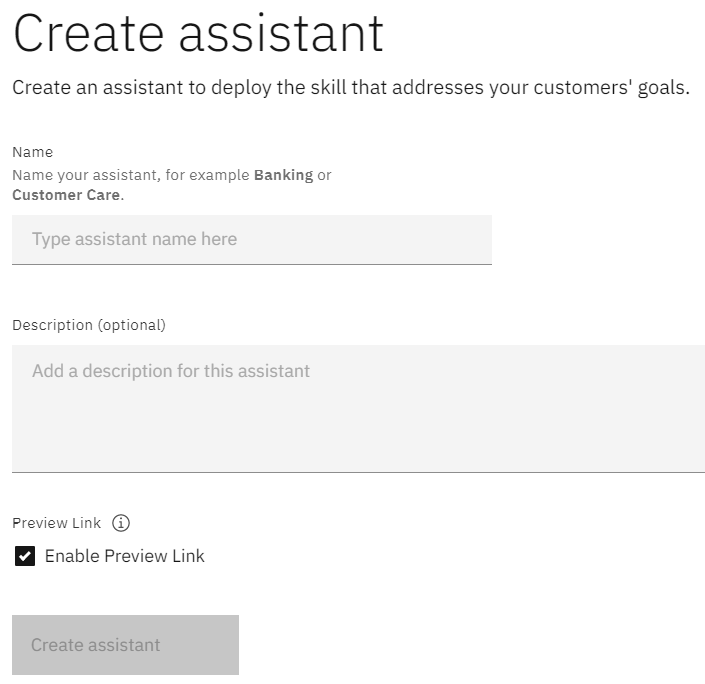
\includegraphics[width=0.75\textwidth]{watson-create}
    \caption{Het aanmaken van een assistent in IBM Watson}
\end{figure}

IBM werkt voor het trainen van zijn assistenten met zogenaamde skills, deze bevatten alles om vragen van klanten te kunnen beantwoorden. Bij IBM Watson wordt er niet per assistent getraind, maar er wordt een skill aangemaakt die kan worden toegevoegd aan de assistent naar keuze. Er kunnen dus meerdere skills aan één assistent toegevoegd worden. Bij het aanmaken van een skill is het noodzakelijk om een naam en een standaardtaal op te geven. Door verschillende skills met verschillende talen toe te voegen aan een assistent, kan er dus ook een meertalige chatbot gemaakt worden.

\begin{figure}[H]
    \label{fig:watson-skill}
    \centering
    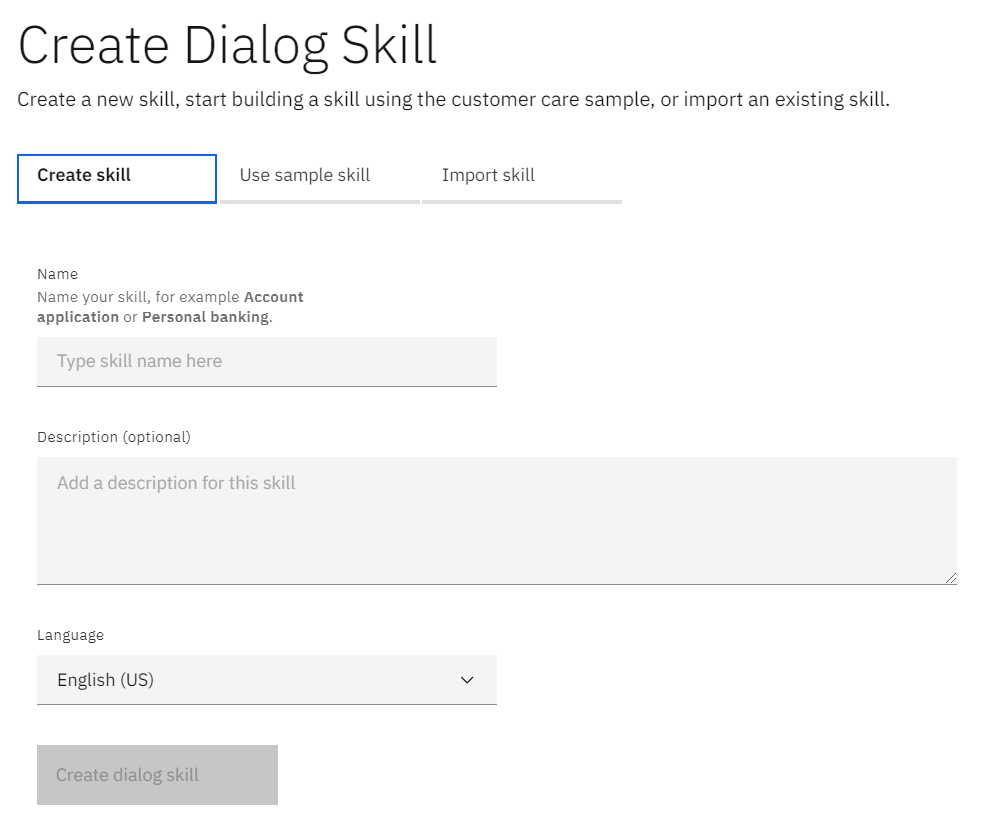
\includegraphics[width=0.75\textwidth]{watson-skill}
    \caption{Het aanmaken van een skill in IBM Watson}
\end{figure}

Eens een skill is aangemaakt, kan het configureren van de skill beginnen. Het toevoegen van een intent is ook hier eenvoudig, want er is enkel een naam en een aantal voorbeeldzinnen nodig. IBM Watson legt geen restricties op het aantal voorbeeldzinnen, maar opnieuw is het aangeraden om er 10-15 te voorzien per intent. Het configureren van intents verschilt ook met de andere platformen, omdat er geen entities toegevoegd kunnen worden aan de intents en aan de voorbeeldzinnen. In de andere platformen moet je zelf aanduiden welke woorden in de zin behoren tot een entity. In onderstaand voorbeeld is het duidelijk dat je 9 augustus niet zelf moet toewijzen aan de entiteit 'datum'. Dat is een functionaliteit die IBM met hun chatbotplatform achter de schermen gaat doen voor de ontwikkelaar. Watson gaat zelf op zoek naar entiteiten in de voorbeeldzinnen zonder dat de ontwikkelaar daar enige tijd in hoeft te stoppen om ze zelf allemaal aan te duiden. Dat betekent dat het proces van het ontwikkelen van een chatbot efficiënter kan verlopen. Watson heeft net zoals bovenstaande platformen een aantal ingebouwde entities waarvoor je niets hoeft te doen. Hoe goed deze methode zal werken, zal blijken uit het experiment.

\begin{figure}[H]
    \label{fig:watson-intent}
    \centering
    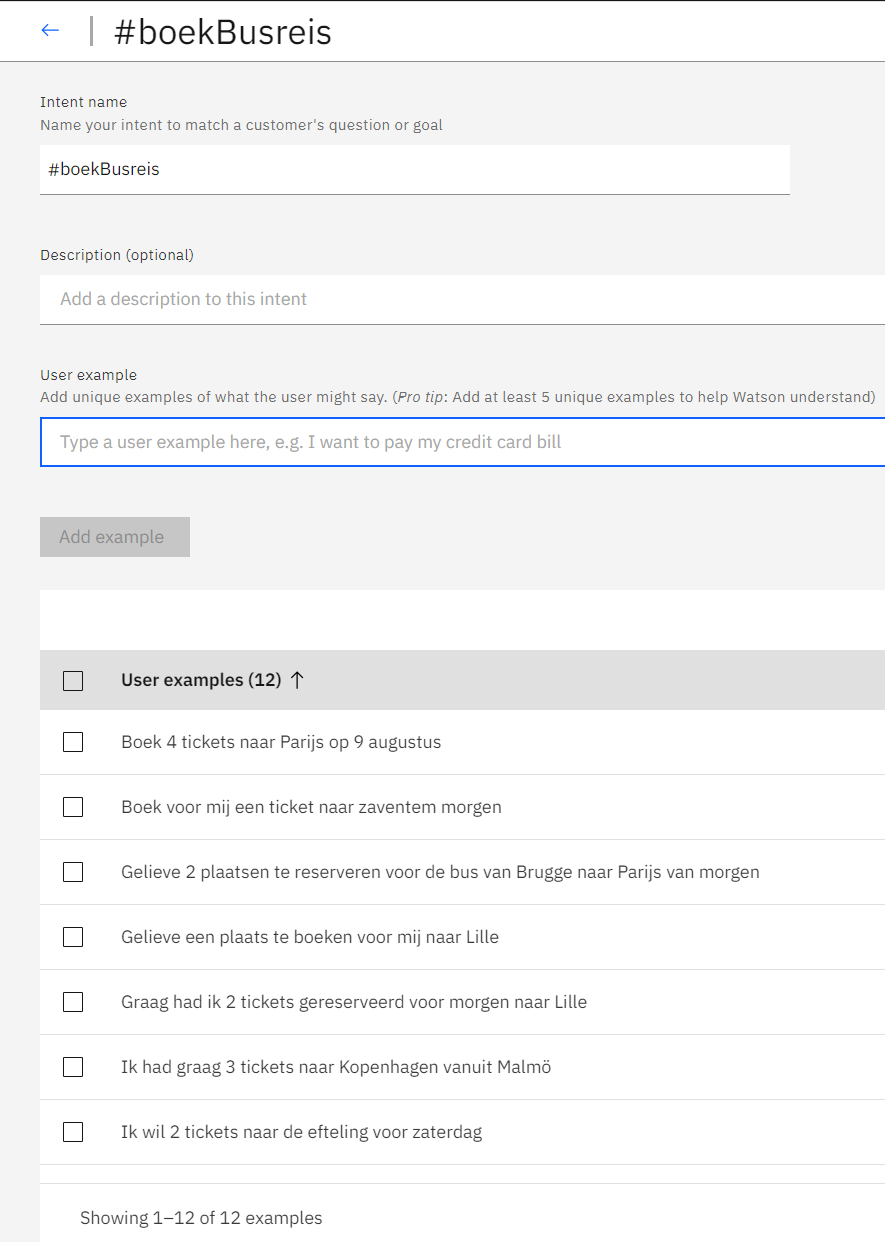
\includegraphics[width=0.75\textwidth]{watson-intent}
    \caption{Het configureren van een intent in IBM Watson}
\end{figure}

In IBM Watson kunnen ook eigen entiteiten toegevoegd worden, dat komt vrijwel volledig overeen met hoe dat gedaan wordt in Dialogflow. Er kunnen waarden voor die entiteit toegevoegd worden alsook synoniemen. Het is ook mogelijk om op basis van patronen entiteiten uit berichten te halen. Het enige verschil met Dialogflow is de manier waarop entiteiten gebruikt worden, want zoals eerder vermeld moet de ontwikkelaar buiten het creëren van de entiteit niets doen om het te gebruiken, de entiteiten moeten niet aangeduid worden in de voorbeeldzinnen in de intents.

\begin{figure}[H]
    \label{fig:watson-entity}
    \centering
    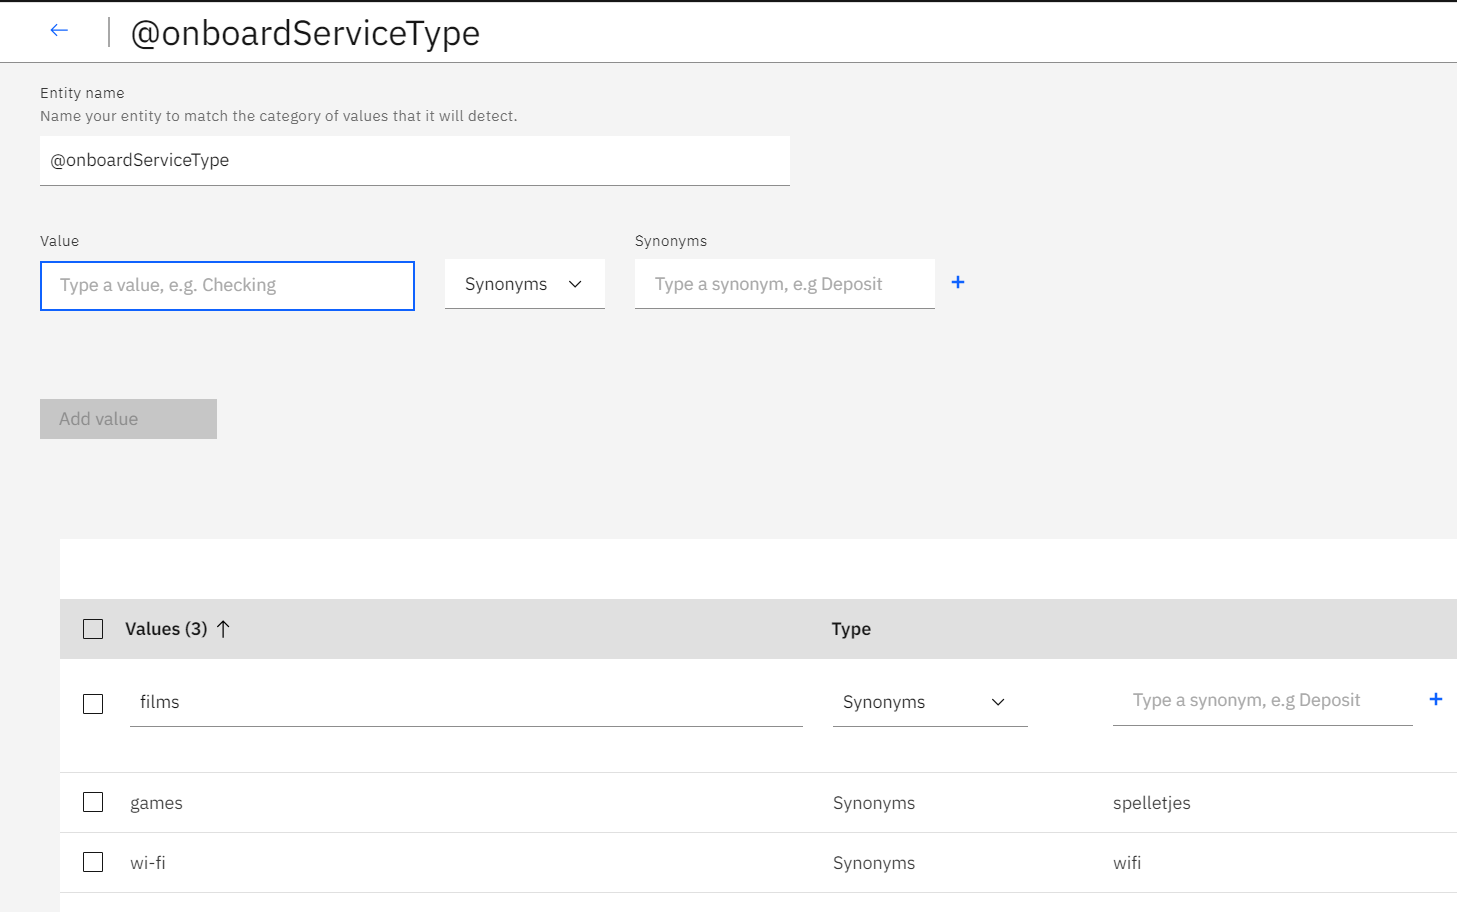
\includegraphics[width=0.9\textwidth]{watson-entity}
    \caption{Het configureren van een entiteit in IBM Watson}
\end{figure}

Het is met IBM Watson ook mogelijk om een volledige conversatieflow van een skill vast te leggen. Als ontwikkelaar kan je verschillende nodes en subnodes toevoegen en die volledig configureren naar eigen wens. Deze nodes kunnen worden uitgevoerd als een intent, contextvariabele of entity herkent wordt door het model. In de nodes kunnen er ook antwoorden voorzien worden die de assistent zal geven, deze functionaliteit zal binnen deze bachelorproef niet beoordeeld worden, omdat dit geen invloed heeft op de prestaties van intent classificatie. Het is immers wel een interessante functionaliteit die een rol kan spelen in het kiezen naar een platform.

\begin{figure}[H]
    \label{fig:watson-dialogen}
    \centering
    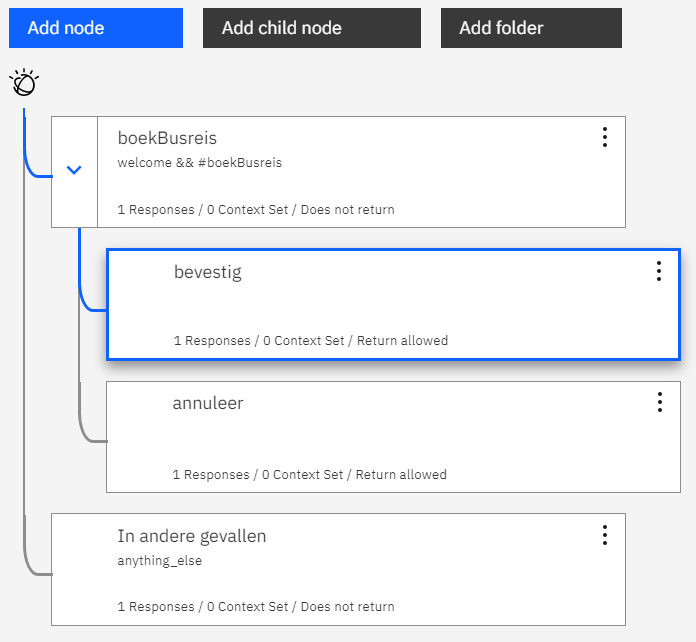
\includegraphics[width=0.75\textwidth]{watson-dialogen}
    \caption{Conversatieflow die zelf samengesteld kan worden in IBM Watson}
\end{figure}

\begin{figure}[H]
    \label{fig:watson-node}
    \centering
    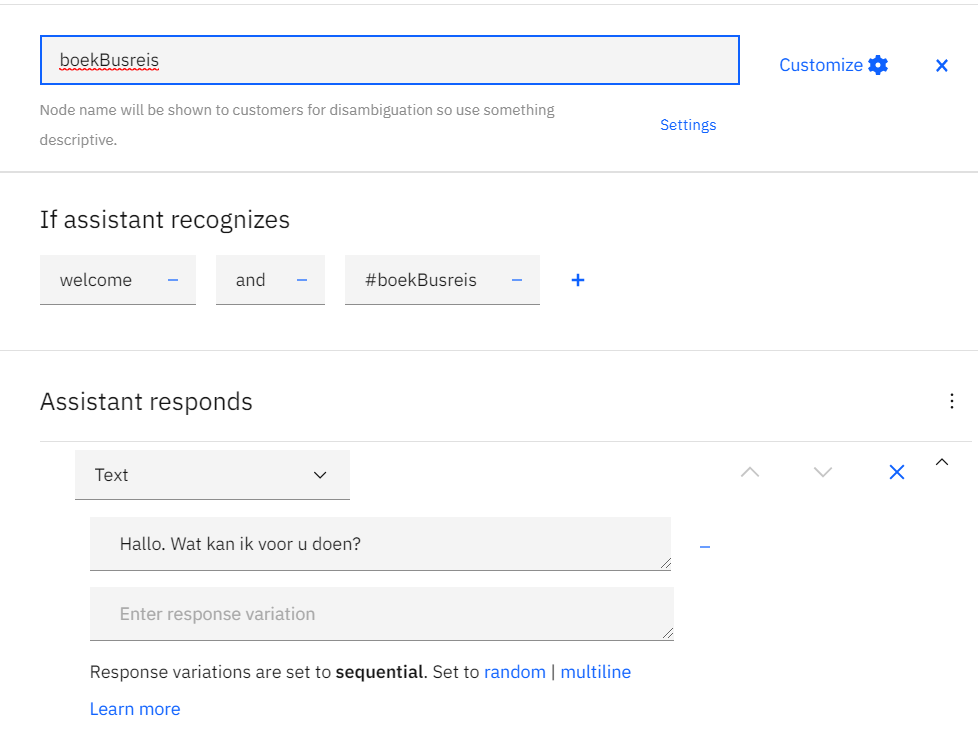
\includegraphics[width=0.75\textwidth]{watson-node}
    \caption{Het configureren van een node van in de conversatieflow in IBM Watson}
\end{figure}

Watson biedt een beperkt aantal ingebouwde integraties aan (Facebook \& Slack), maar het is wel mogelijk om zelf een applicatie te bouwen die gebruik maakt van de aangeboden API.

De gebouwde skills kunnen ook getest worden via een ingebouwde conversatiemodule. Bij het versturen van een bericht, wordt er een antwoord gegeven waarin duidelijk wordt aangegeven welke intent is herkend.

\begin{figure}[H]
    \label{fig:watson-test}
    \centering
    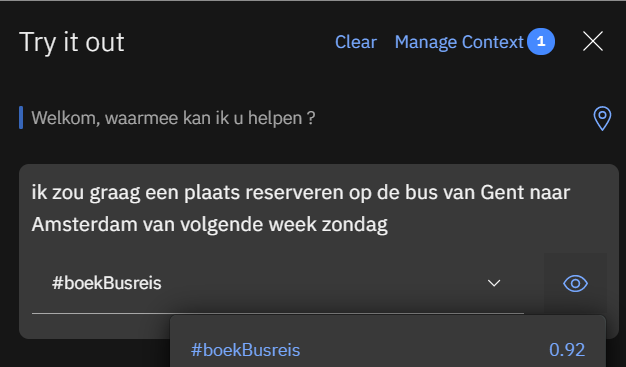
\includegraphics[width=0.65\textwidth]{watson-test}
    \caption{Het testen van IBM Watson via de ingebouwde interface}
\end{figure}

\subsection{LUIS}
\label{subsec:werking-platformen-luis}

LUIS staat voor Language Understanding Intelligent Service en is de NLU-tool van Microsoft en is onderdeel van het Microsoft Azure cloud service platform. Dat is opnieuw goed vergelijkbaar met Google Cloud en met IBM Cloud. LUIS is een pure NLU-tool en kan dus niet worden gebruikt om dialooglogica uit te werken. Daarvoor kan het geïntegreerd worden met het Microsoft Bot Framework, dat ook onderdeel is van Azure en wel op berichten van eindgebruikers kan antwoorden en dialogen kan voeren. LUIS is ook onderdeel van dat framework, het wordt gewoon gezien als een individuele dienst. Het creëren van een applicatie met LUIS is ook eenvoudig, doordat er een gebruiksvriendelijke interface voorzien is, net zoals alle voorgaande platformen. Om een applicatie aan te maken heb je enkel een Microsoft account nodig en moet je een naam en taal selecteren.

\begin{figure}[H]
    \label{fig:luis-create}
    \centering
    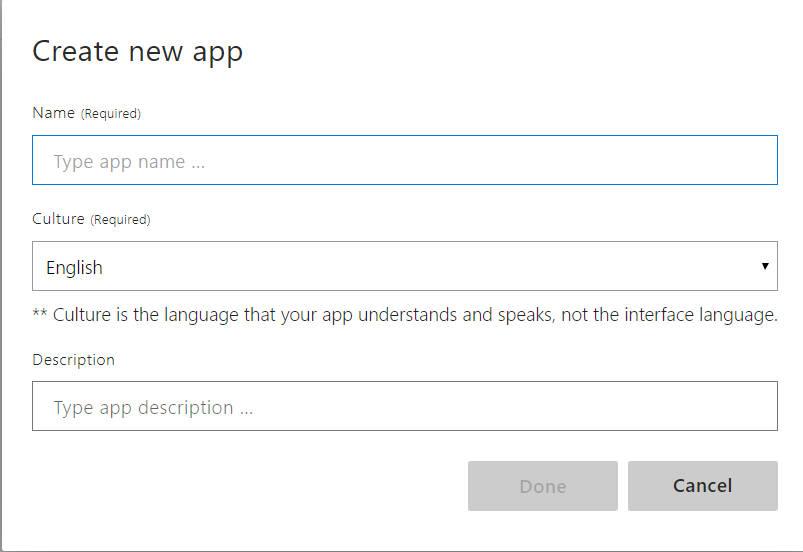
\includegraphics[width=0.65\textwidth]{luis-create}
    \caption{Het aanmaken van een applicatie via LUIS}
\end{figure}

Het toevoegen en configureren van intents is vrij gelijkaardig aan de manier die Dialogflow toepast. Het is opnieuw belangrijk dat er genoeg voorbeeldzinnen per intent zijn om ervoor te zorgen dat de applicatie goed getraind kan worden. LUIS gebruikt de naam 'utterances' om voorbeeldzinnen te beschrijven. Bij LUIS is het opnieuw vereist om zelf aan te geven welke woorden entiteiten zijn, dit kunnen zowel systeementiteiten als zelfgemaakte entiteiten zijn.

\begin{figure}[H]
    \label{fig:luis-intent}
    \centering
    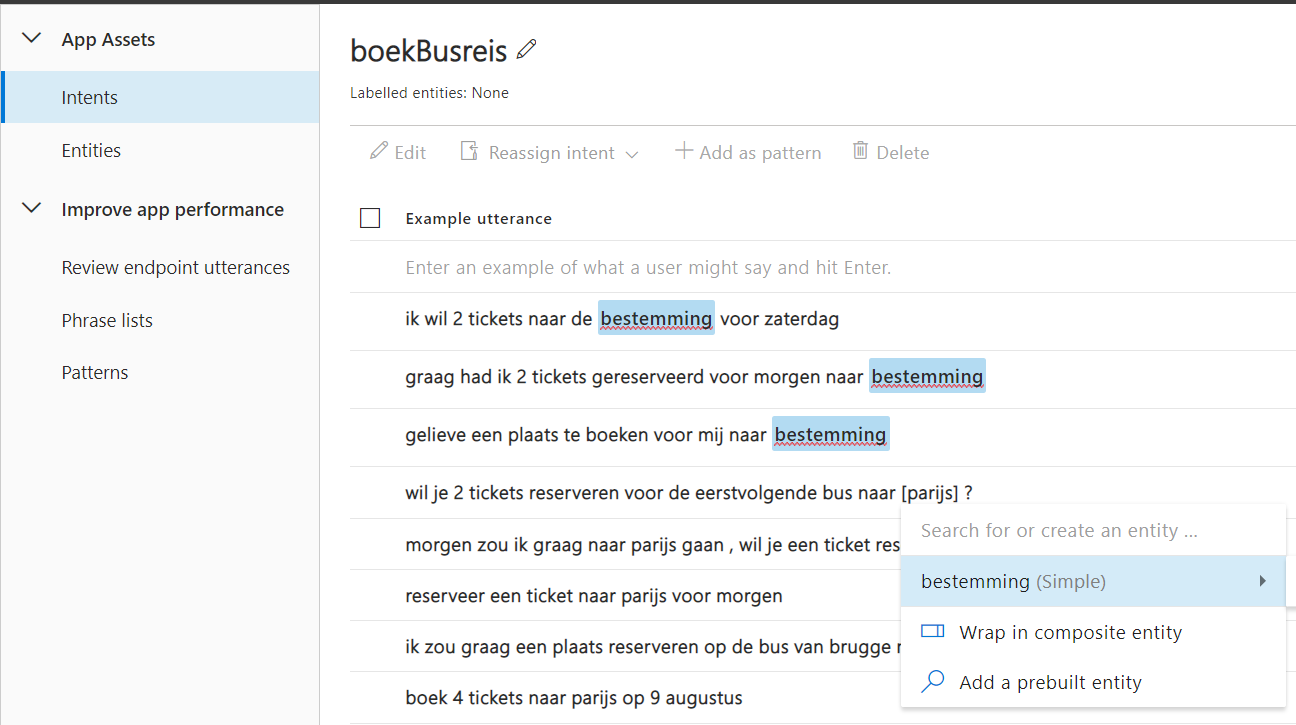
\includegraphics[width=0.85\textwidth]{luis-intent}
    \caption{Het configureren van een intent in LUIS}
\end{figure}

LUIS biedt een grote hoeveelheid vooraf gebouwde intents, entities en zelfs domeinen aan. Domeinen zijn een verzameling van vooraf getrainde modellen van intents en entities die samenwerken. Dit wordt niet ondersteund in het Nederlands en zal daarom niet verder worden besproken. Verder is het mogelijk om zelf entities toe te voegen en te gebruiken. Indien je als ontwikkelaar systeementiteiten wil gebruiken, is het wel noodzakelijk om die eerst toe te voegen, want indien je dit niet doet, zal het niet mogelijk zijn om ze te gebruiken in de utterances. Er zijn verschillende soorten entiteittypes om uit te kiezen. Opvallend is wel dat er bij LUIS geen waarden voor de entiteit moeten meegegeven worden. Dat betekent dat het niet nodig is om bijvoorbeeld de waarden 'morgen' of 'vrijdag' toe te kennen aan de entiteit 'datum'.

\begin{figure}[H]
    \label{fig:luis-entity}
    \centering
    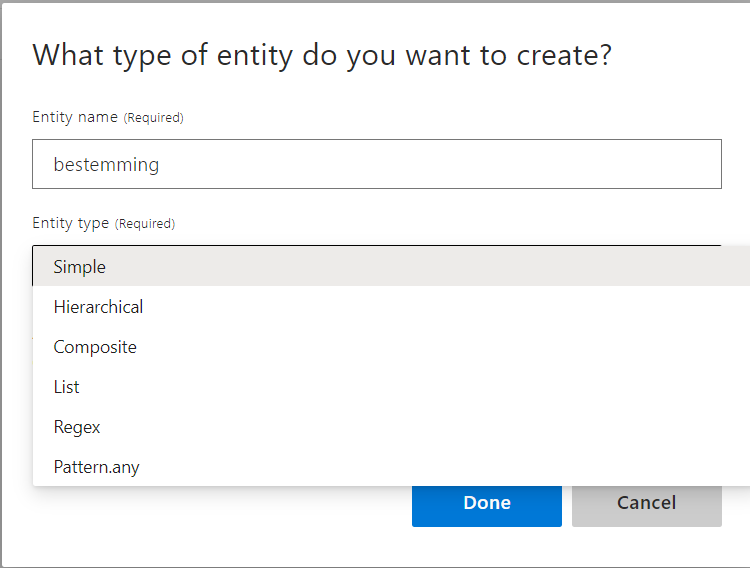
\includegraphics[width=0.65\textwidth]{luis-entity}
    \caption{Het aanmaken van een entiteit binnen LUIS}
\end{figure}

Met LUIS is het net zoals bij Dialogflow mogelijk om als ontwikkelaar eerdere berichten die eindgebruikers hebben gestuurd naar de applicatie te valideren. Het enige verschil bij LUIS is dat enkel utterances waarover hij onzeker is, nog moeten gevalideerd worden door de ontwikkelaar, de rest gebeurt automatisch.

\begin{figure}[H]
    \label{fig:luis-validate}
    \centering
    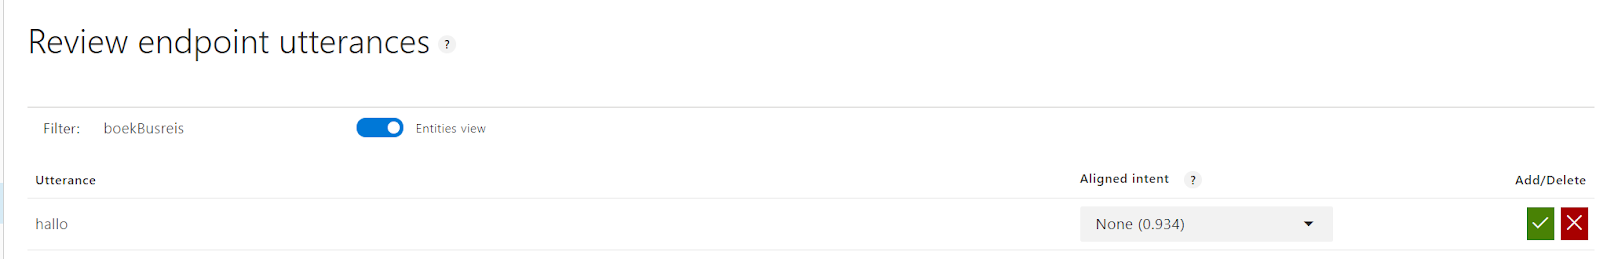
\includegraphics[width=\textwidth]{luis-validate}
    \caption{Het beoordelen van utterances waarover LUIS onzeker is}
\end{figure}

Voor LUIS getest kan worden, is het verplicht om het model te trainen, dit moet manueel gebeuren. Indien je dit niet doet, is het niet mogelijk om berichten te sturen naar de chatbot.

\begin{figure}[H]
    \label{fig:luis-train}
    \centering
    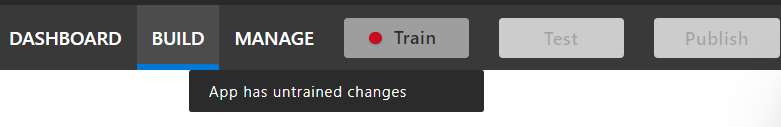
\includegraphics[width=0.65\textwidth]{luis-train}
    \caption{Het manueel trainen van de LUIS applicatie}
\end{figure}

Eens de applicatie getraind is, kan er getest worden, dit kan gebeuren via een ingebouwde module. Bij het versturen van een bericht naar de gebouwde LUIS app, krijgt de gebruiker informatie over welke intent herkend is.
Het is duidelijk zichtbaar welke entities herkend zijn. Ook zal LUIS automatisch een sentimentanalyse uitvoeren, daarbij wordt aangegeven hoe positief of negatief LUIS dit bericht interpreteert.

\begin{figure}[H]
    \label{fig:luis-test}
    \centering
    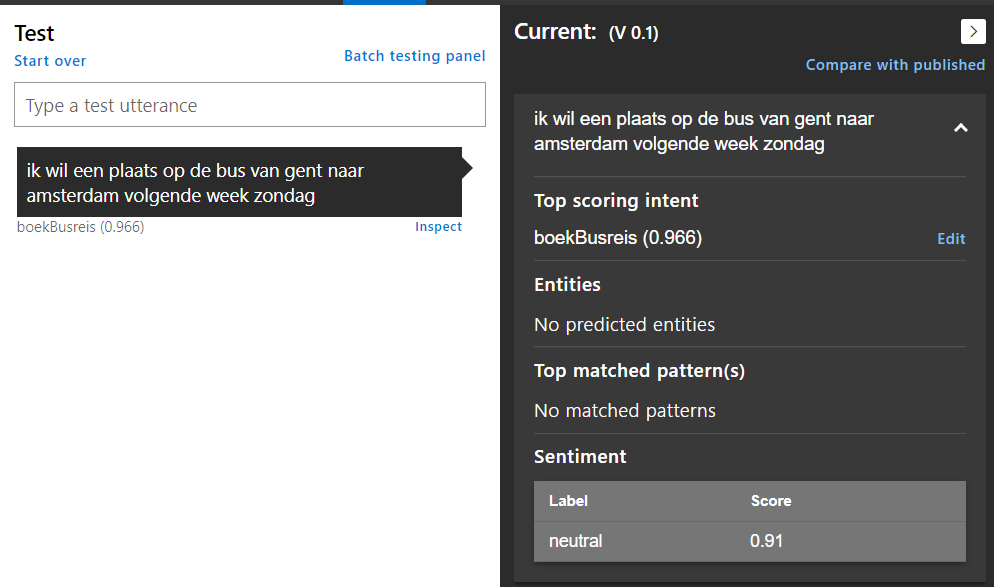
\includegraphics[width=0.75\textwidth]{luis-test}
    \caption{Het testen van een LUIS applicatie}
\end{figure}

\subsection{Wit.ai}
\label{subsec:werking-platformen-wit}

Wit.ai is de NLU-tool van Facebook en is volledig gratis te gebruiken. Het heeft net zoals de vorige platformen een eenvoudige grafische user interface die gebruikt kan worden. Het enige dat je nodig hebt om aan de slag te gaan met Wit.ai is een Github account of een Facebook account. Het staat volledig gratis gehost op het internet en kan via de API bereikt worden. Het bevat geen mogelijkheid om dialogen te configureren en antwoorden in te stellen. Indien je dit wenst, moet er zelf een applicatie worden ontwikkeld die gebruik maakt van de aangeboden API.

Het aanmaken van een applicatie binnen Wit.ai is heel erg eenvoudig, een naam en een standaardtaal zijn de enige vereisten. Het is ook mogelijk om een applicatie te importeren van een backup en er is de keuze om de data die verwerkt wordt in de applicatie te delen met de volledige community of niet.

\begin{figure}[H]
    \label{fig:wit-create}
    \centering
    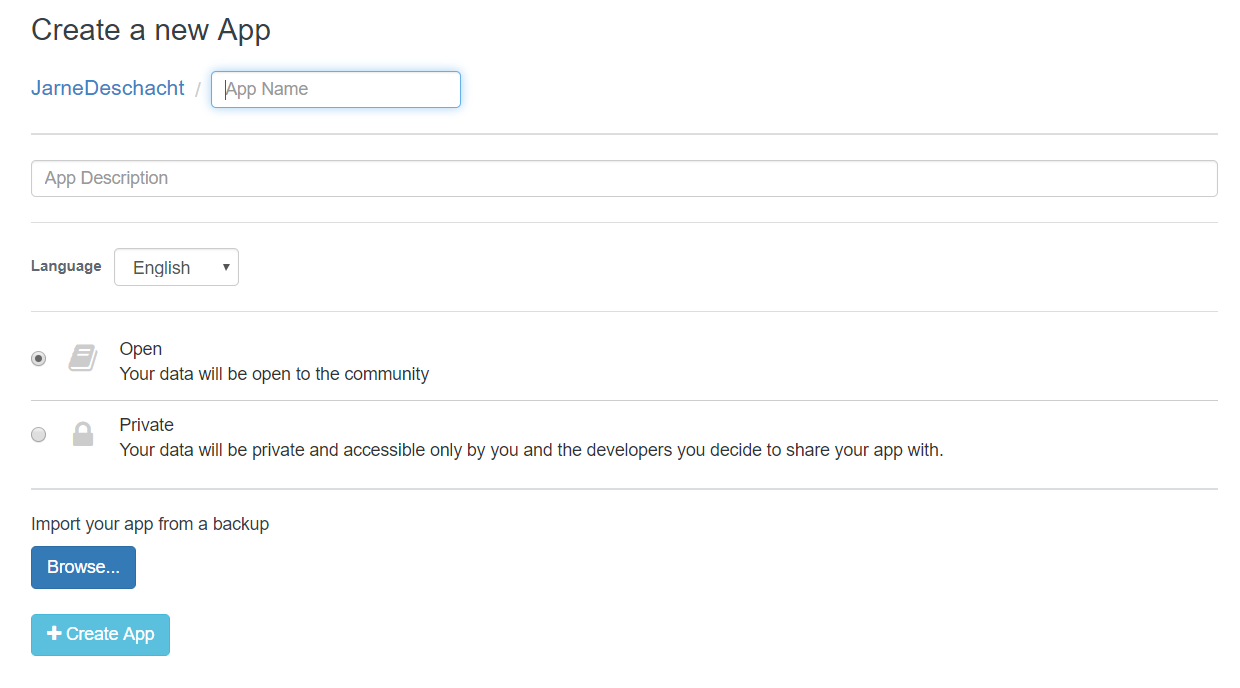
\includegraphics[width=0.75\textwidth]{wit-create}
    \caption{Het aanmaken van een applicatie in Wit.ai}
\end{figure}

Eenmaal de applicatie aangemaakt is, kan het trainen beginnen. De werking van intents en entities binnen Wit.ai wijkt af van hoe de andere platformen hiermee omgaan. Binnen Wit.ai bestaan er enkel entities, geen intents, intents worden gezien als een instantie van een entity. Parameterwaarden worden dus ook als entities gezien, net zoals intents. Bij het toevoegen van nieuwe trainingsdata, moet dus altijd minstens één entity toegevoegd worden, namelijk de entity ‘intent’. Net zoals bij andere entities kunnen dan verschillende waarden toegevoegd worden, deze waarden komen dan overeen met de namen van de mogelijke intents. Dit klinkt erg verwarrend, maar onderstaande voorbeelden verduidelijken deze werking.

\begin{figure}[H]
    \label{fig:wit-train}
    \centering
    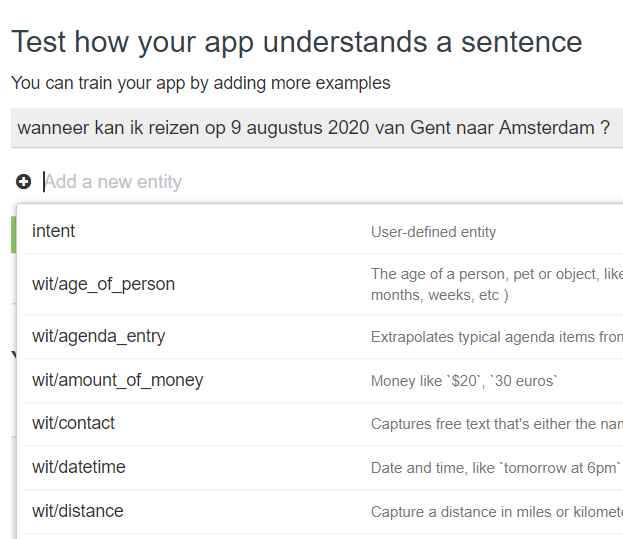
\includegraphics[width=0.65\textwidth]{wit-train}
    \caption{Het trainen van een Wit.ai applicatie}
\end{figure}

\begin{figure}[H]
    \label{fig:wit-intent}
    \centering
    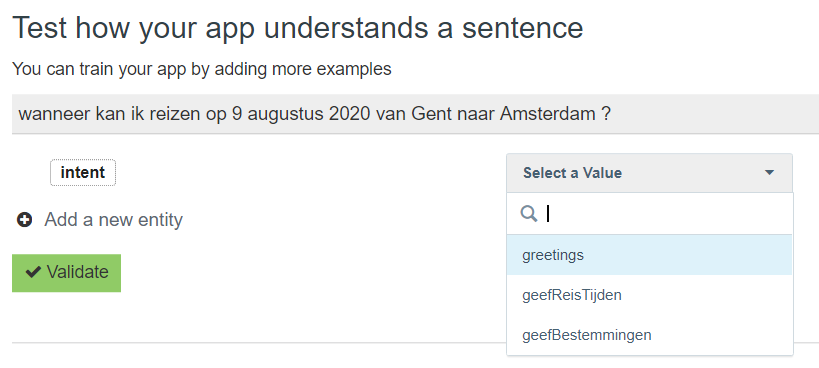
\includegraphics[width=0.65\textwidth]{wit-intent}
    \caption{Het kiezen van een intent bij het trainen in Wit.ai}
\end{figure}

Net zoals bij de andere platformen is het mogelijk om extra entities toe te wijzen aan woorden in de voorbeeldzinnen. Er is keuze uit een aantal voorgedefinieerde entities, maar het is ook mogelijk om zelf entities aan te maken en te gebruiken.

\begin{figure}[H]
    \label{fig:wit-entity}
    \centering
    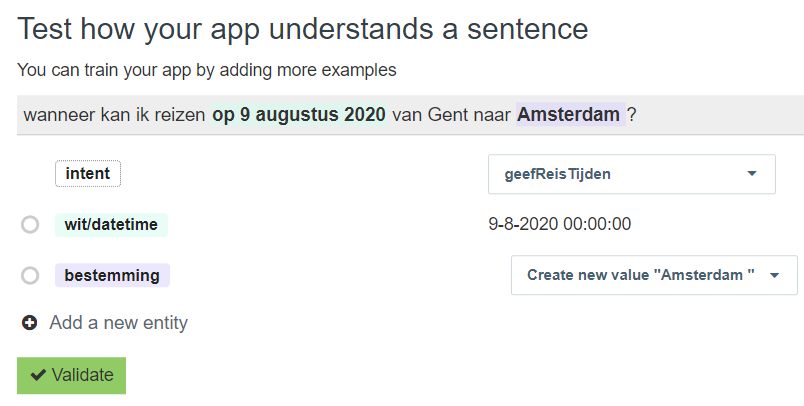
\includegraphics[width=0.65\textwidth]{wit-entity}
    \caption{Het aanduiden van entities in een voorbeeldzin in Wit.ai}
\end{figure}

Het is opnieuw mogelijk om extra waarden en synoniemen toe te voegen aan de entities, net zoals in de andere platformen.

\begin{figure}[H]
    \label{fig:wit-intent-manage}
    \centering
    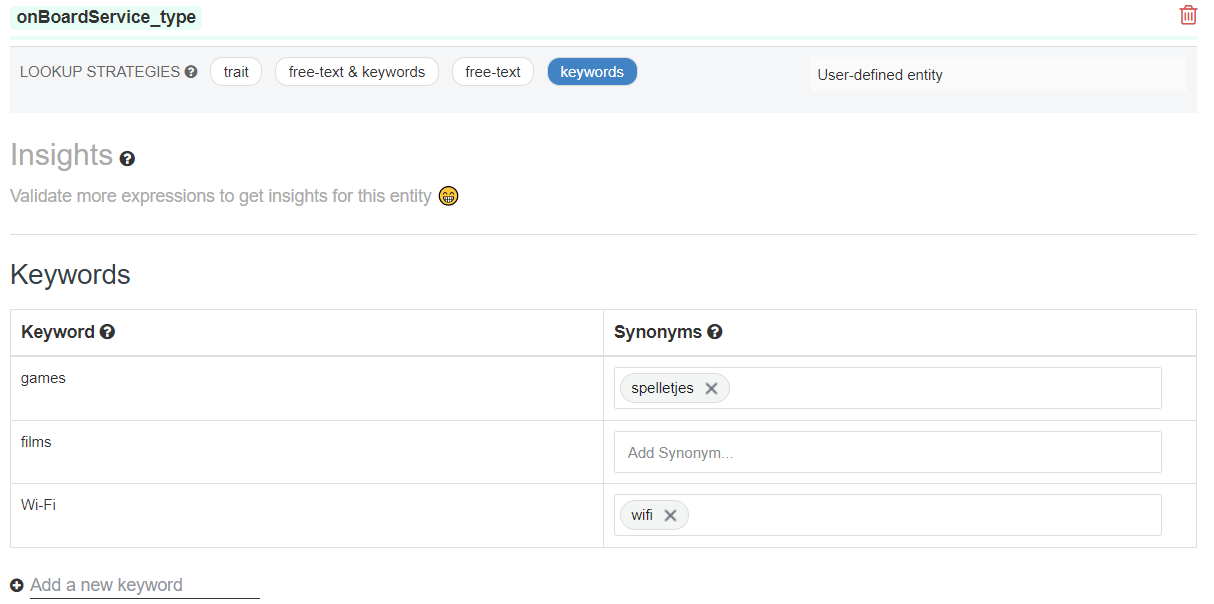
\includegraphics[width=0.85\textwidth]{wit-entity-manage}
    \caption{Het configureren van entities in Wit.ai}
\end{figure}

Wit.ai bevat geen module om de gebouwde applicatie te valideren, het biedt wel een API aan om dat te doen. Deze API zal later ook gebruikt worden om training te automatiseren, maar meer hierover in een latere sectie. Om gebruik te maken van deze API, werd een tool, genaamd Postman, gebruikt. Daarmee kan eenvoudig een verzoek naar de server van Wit.ai verstuurd worden om de chatbot te testen.

\begin{figure}[H]
    \label{fig:wit-test}
    \centering
    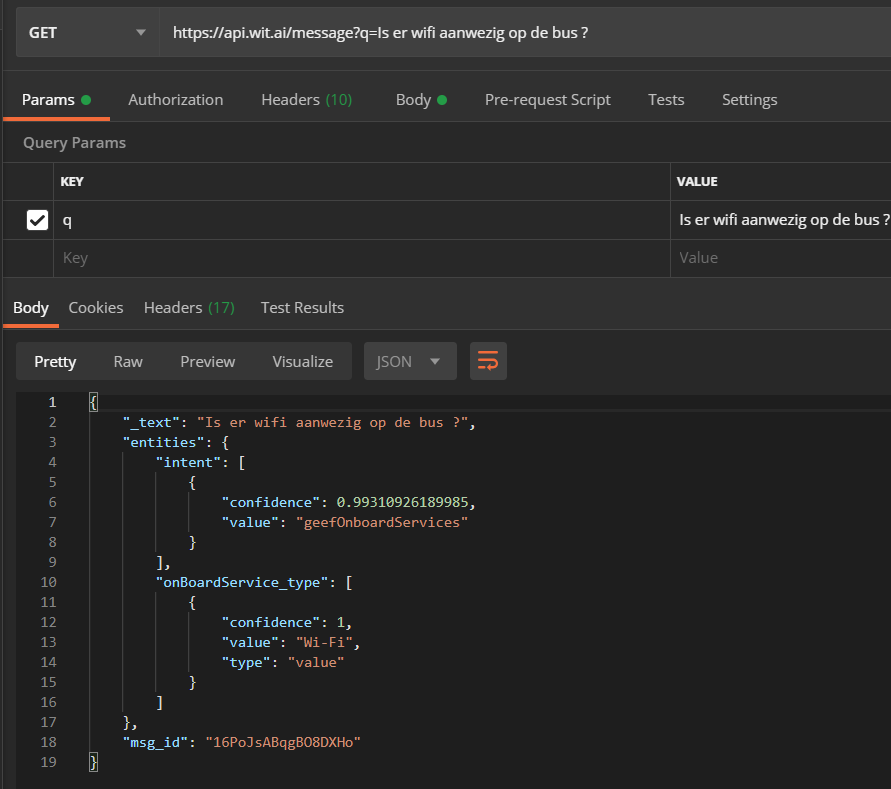
\includegraphics[width=0.75\textwidth]{wit-test}
    \caption{Voorbeeld van een request met Postman naar de server van Wit.ai om de applicatie te testen}
\end{figure}

\subsection{Rasa}
\label{subsec:werking-platformen-rasa}

Zoals eerder vermeld is Rasa een tool die qua gebruik sterk afwijkt van de eerder besproken platformen, omdat het meer technische kennis vereist in vergelijking met de andere. Om gebruik te maken van Rasa moet het platform eerst lokaal gedownload worden. De makkelijkste manier om dit te doen is door gebruik te maken van Pip. Pip is een tool die gebruikt wordt om softwarepakketten die geschreven zijn in de programmeertaal Python te installeren. Rasa biedt in tegenstelling tot de eerder besproken platformen ook geen grafische user interface (GUI) aan. Dit betekent dat alles in de command line interface (CLI) moet gebeuren. De CLI is de grote tegenhanger van de GUI en is een andere manier om met software te communiceren, want de CLI wordt enkel gebruikt op basis van tekstcommando's.

\begin{figure}[H]
    \label{fig:rasa-install}
    \centering
    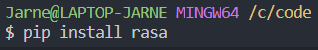
\includegraphics[width=0.35\textwidth]{rasa-install}
    \caption{Voorbeeld van een commando binnen de CLI waarbij Rasa geïnstalleerd wordt door middel van Pip}
\end{figure}

Eens Rasa succesvol geïnstalleerd is, kan er een project opgestart worden, dat kan met het commando ‘rasa init’. Daarbij zal er de vraag komen in welke map het project geïnstalleerd moet worden en of dat er een voorbeeldmodel getraind moet worden. Eens dat gelukt is, kan de configuratie van de chatbot beginnen.

\begin{figure}[H]
    \label{fig:rasa-create}
    \centering
    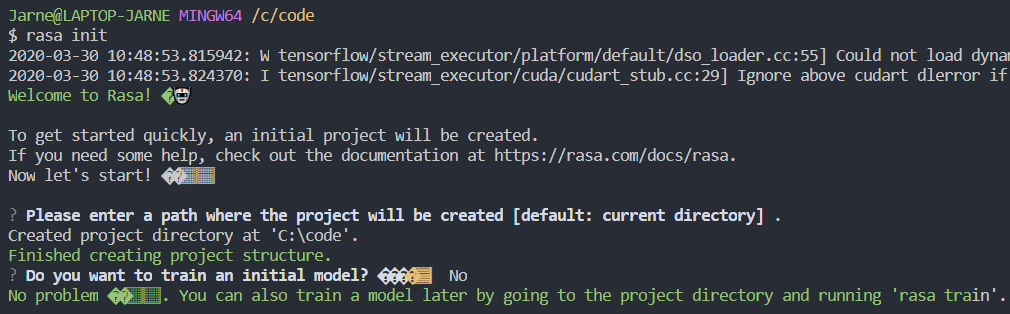
\includegraphics[width=\textwidth]{rasa-create}
    \caption{Het creëren van een project met Rasa in de CLI}
\end{figure}

Rasa bestaat uit twee hoofdmodules, Rasa NLU en Rasa Core. De focus binnen dit onderzoek zal liggen op Rasa NLU. Dit is de intentclassificatiemodule van Rasa die nodig is om het begrijpend vermogen van een chatbot te evalueren. Rasa Core is essentieel voor het vastleggen van dialogen en antwoorden richting de eindgebruiker. Rasa werkt zoals de andere platformen ook met intents en entities. Het configureren ervan gebeurt in een bestand genaamd ‘nlu.md’ dat aangemaakt wordt bij het creëren van een project. Daarin kunnen heel eenvoudig intents met bijhorende voorbeeldzinnen toegevoegd worden. Entities moeten binnen Rasa ook niet vooraf gedefinieerd worden, ze kunnen direct aangeduid worden in de voorbeeldzinnen en Rasa doet de rest. Het is ook mogelijk om synoniemen te voorzien voor entities en om entities te herkennen op basis van patronen.

\begin{figure}[H]
    \label{fig:rasa-intent}
    \centering
    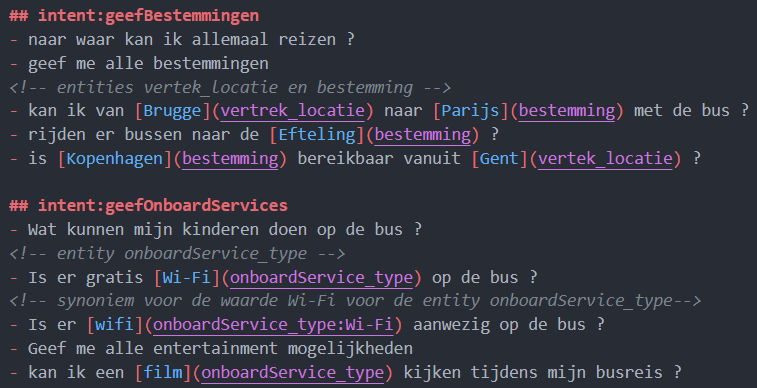
\includegraphics[width=0.85\textwidth]{rasa-intent}
    \caption{Het configureren van de intents en voorbeeldzinnen met entities in Rasa}
\end{figure}

Het moeilijkste deel bij het gebruik van Rasa is het vastleggen van de configuratie van Rasa NLU en Rasa Core. Rasa kan door de ontwikkelaar volledig op maat van een project afgesteld worden. Berichten die via Rasa binnenkomen, worden verwerkt door softwarepakketten die je als ontwikkelaar zelf kunt kiezen. Dit wordt in de andere platformen achter de schermen voor ons gedaan, waardoor er hier niet altijd controle over is. Binnen deze bachelorproef wordt er beperkt tot de Nederlandse taal, dus moeten er componenten worden gebruikt die Nederlands ondersteunen. De configuratie vastleggen kan opnieuw via een bestand (config.yml) die bij het creëren aangemaakt werd. Bij het vastleggen van de configuratie werden de aanbevelingen vanuit de officiële documentatie gebruikt. Het voornaamste is dat er componenten worden gebruikt die overweg kunnen met de Nederlandse taal. Voor entityherkenning werd eveneens een specifieke component gebruikt, dat is nodig om entiteiten zoals locaties, datums, tijdstippen, etc. te kunnen extraheren. Deze component werd enkel gebruikt voor experimenten waarbij entities nodig zijn. De configuratie van Rasa Core heeft eveneens tal van mogelijkheden, maar dit behoort niet tot de scope van deze bachelorproef. Over alle opties en mogelijkheden van Rasa, kan een volledige bachelorproef geschreven worden. 

\begin{figure}[H]
    \label{fig:rasa-config}
    \centering
    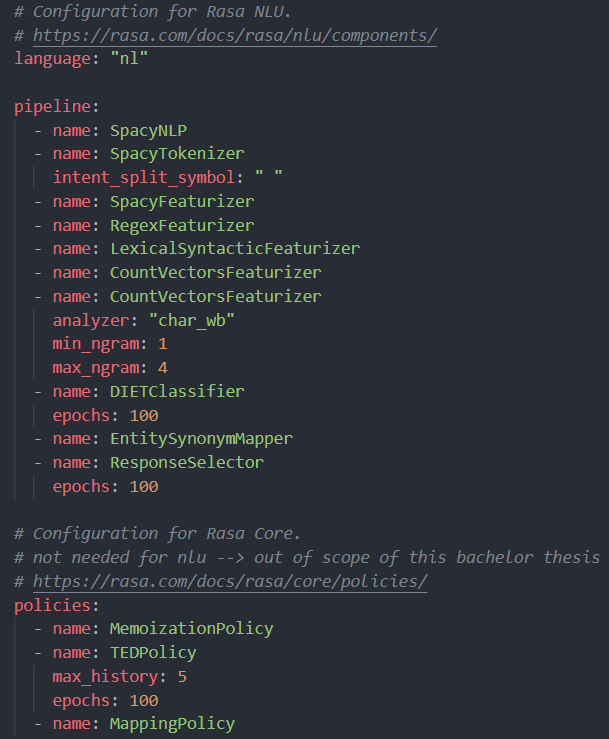
\includegraphics[width=0.80\textwidth]{rasa-config}
    \caption{Configuratie van Rasa NLU}
\end{figure}

Met Rasa Core is het zoals eerder vermeld mogelijk om dialogen en antwoorden naar eindgebruikers te configureren. Rasa Core wordt standaard mee geïnstalleerd, maar zal binnen deze bachelorproef niet verder gebruikt en besproken worden.

Eens de configuratie van Rasa is gebeurd en er een aantal intents toegevoegd zijn, kan het trainen en testen van de chatbot gebeuren. Het is mogelijk om afzonderlijke modules te trainen. Om enkel de NLU-module te trainen, moet er in de CLI het commando ‘rasa train nlu’ uitgevoerd worden.

\begin{figure}[H]
    \label{fig:rasa-train}
    \centering
    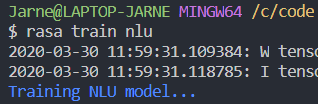
\includegraphics[width=0.5\textwidth]{rasa-train}
    \caption{Het trainen van de NLU module van Rasa}
\end{figure}

Als de training succesvol afgerond is, dan is het mogelijk om de NLU-module te testen. Dit kan gedaan worden door het commando ‘rasa shell nlu’ uit te voeren. Daarbij wordt een lokale server opgestart waarnaar berichten kunnen worden gestuurd en intents en entities herkend kunnen worden. Indien deze server publiek toegangelijk moet zijn, kan het eventueel op Google Cloud, AWS of Microsoft Azure gezet worden. Bij antwoord van de server is de herkende intent zichtbaar, alsook de herkende entities. Bij de intent staat er aangegeven hoe zeker de applicatie is van de intent die hij heeft gekozen, in onderstaand voorbeeld is dit 99.985\%, wat goed is, want meestal ligt dit percentage lager.

\begin{figure}[H]
    \label{fig:rasa-test}
    \centering
    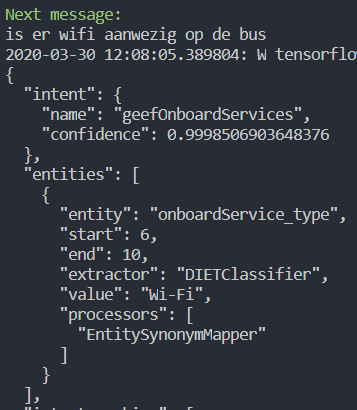
\includegraphics[width=0.5\textwidth]{rasa-test}
    \caption{Voorbeeld van een response bij het sturen van een bericht naar de NLU-module}
\end{figure}

\section{Automatisatie}
\label{sec:automatisatie}

Tot nu toe werd er telkens via een user interface rechtstreeks gewerkt op de verschillende platformen om bijvoorbeeld een model te trainen of te testen. Deze manier van werken is goed, maar zal bij grote hoeveelheden data heel veel tijd in beslag nemen. Stel je maar voor dat er 10 000 voorbeeldzinnen  en 100 intents zijn en dat dit via de user interface moet ingevoerd worden. Volgens 5-fold cross validation moeten er dan een aantal keer 8000 zinnen getraind worden en 2000 zinnen getest. Dit zou volgens de werking in de sectie hierboven beschreven enorm veel tijd in beslag nemen en onbeheersbaar worden. Om dit op te lossen bieden de platformen een oplossing aan genaamd een API. Dit is een andere manier om te communiceren met de platformen. Het is mogelijk om vanuit een eigen geprogrammeerde applicatie te communiceren met deze API’s en eigenlijk van volledig dezelfde functionaliteiten gebruik te maken als hierboven beschreven, zonder dat er rechtstreeks op de platformen moet gewerkt worden. Dit betekent dat we zelf de code kunnen schrijven die het volledige proces van het trainen en het valideren van de platformen kan automatiseren door gebruik te maken van die API’s. De platformen bieden ook een andere oplossing voor dit probleem aan, genaamd SDK's. Dat staat voor Software Development Kit en dat is een tool die de werking met de platformen vanuit eigen geschreven code eenvoudiger maakt. Achterliggend zullen SDK's ook gebruik maken van de API's, maar de ontwikkelaar moet daar zelf minder voor instaan. Binnen deze bachelorproef werd verder enkel nog gebruik gemaakt van de verschillende API’s en SDK's. Dit met het resultaat dat het experiment veel sneller uitgevoerd en herhaald kan worden zonder dat dit manueel via de user interface van de platformen moet gebeuren.

Alle automatisatiescrips zijn geschreven in de programmeertaal Python en maken gebruik van de API’s en SDK's aangeboden door de verschillende platformen. Er zijn scripts geschreven voor zowel het trainen, als het testen van de verschillende platformen voor alle experimenten die uitgevoerd zijn. Voor het toepassen van cross validation werd eveneens een script geschreven die de initiële dataset willekeurig verdeeld in vijf verschillende delen en daarmee dan de juiste train-en-test datasets mee zal vormen zoals beschreven in sectie 3.3. Daarvoor werd gebruik gemaakt van Scikit-learn, een softwarepakket dat verschillende functionaliteiten voor machine learning aanbiedt voor de programmeertaal Python. Scikit-learn bevat een module die cross validation zal uitvoeren \autocite{sklearn2020}. De gevormde datasets worden weggeschreven in bestanden die door de andere scripts gebruikt worden voor het trainen en het valideren.

\begin{figure}[H]
    \label{fig:code-kfold}
    \centering
    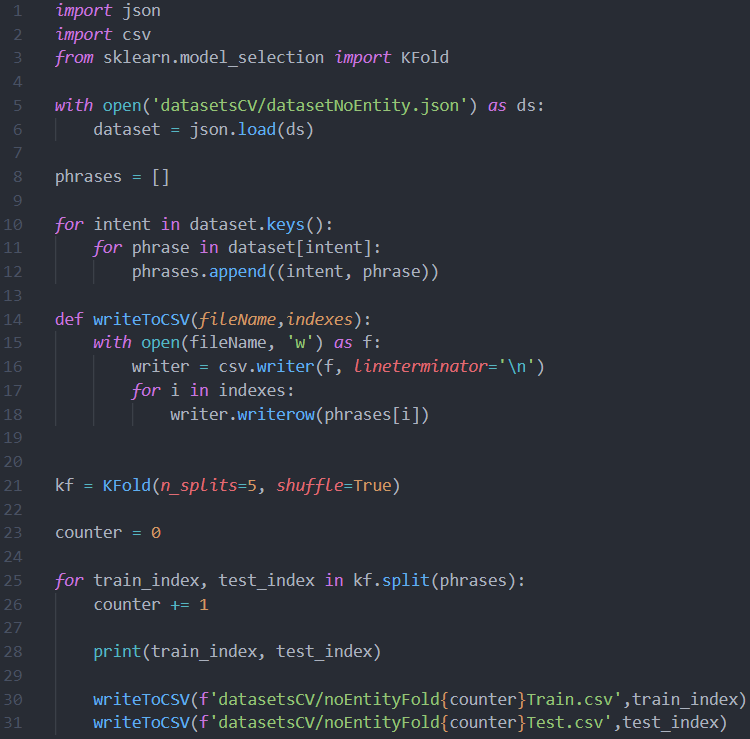
\includegraphics[width=\textwidth]{code-kfold}
    \caption{Script voor het uitvoeren van cross validation op een initiële dataset en de gevormde datasets weg te schrijven naar nieuwe bestanden om gebruikt te kunnen worden door andere train-en-validatie scripts}
\end{figure}

\begin{figure}[H]
    \label{fig:code-validatie}
    \centering
    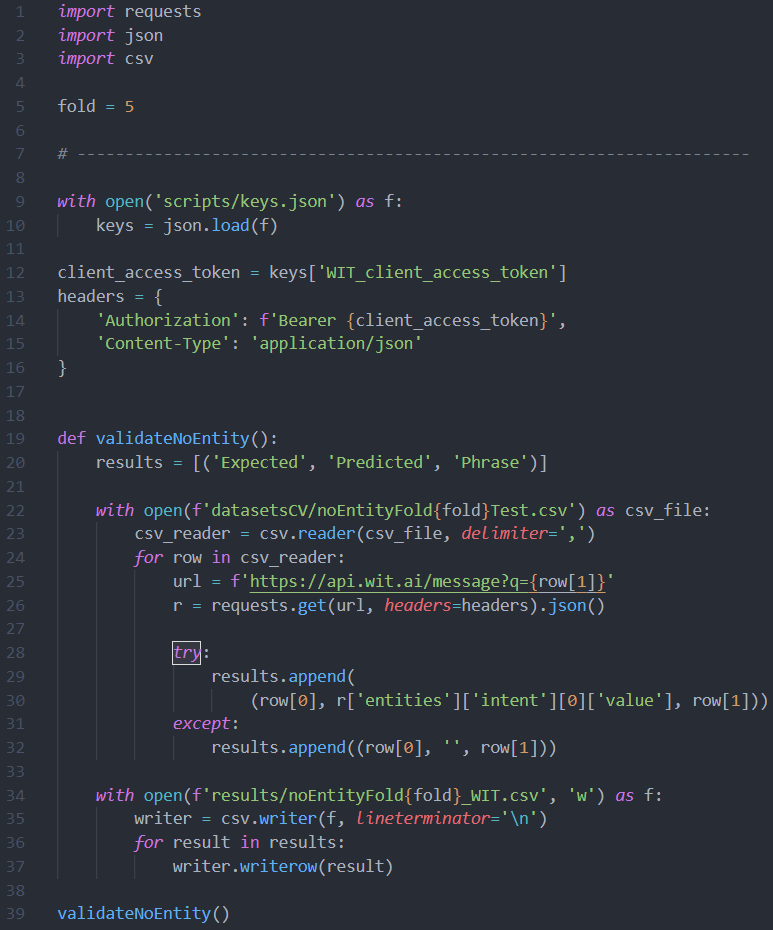
\includegraphics[width=\textwidth]{code-test}
    \caption{Voorbeeld van een Python script waarbij intentherkenning zonder entities van Wit.ai wordt gevalideerd door middel van een dataset van testzinnen en waarbij de resultaten worden weggeschreven naar een nieuw bestand}
\end{figure}



























% Voeg hier je eigen hoofdstukken toe die de ``corpus'' van je bachelorproef
% vormen. De structuur en titels hangen af van je eigen onderzoek. Je kan bv.
% elke fase in je onderzoek in een apart hoofdstuk bespreken.

%\input{...}
%\input{...}
%...

%%=============================================================================
%% Conclusie
%%=============================================================================

\chapter{Resultaten}
\label{ch:resultaten}

\section{Intentherkenning zonder het gebruik van entities}
\label{intent}

Bij het eerste en belangrijkste experiment werden geen entities gebruikt in de dataset en werd puur beoordeeld op intentherkenning. Elk platform is uitgebreid getest door middel van 5-fold cross validation. Elk platform is dus 5 keer gebouwd, getraind en getest geweest om een objectief beeld te krijgen van hoe goed elk platform de juiste intent kan herkennen bij een specifieke input. Van alle resultaten werden confusion matrices opgesteld en werden de precision, recall en f-scores berekent.

\begin{figure}[H]
    \label{fig:confusion-matrix-watson}
    \centering
    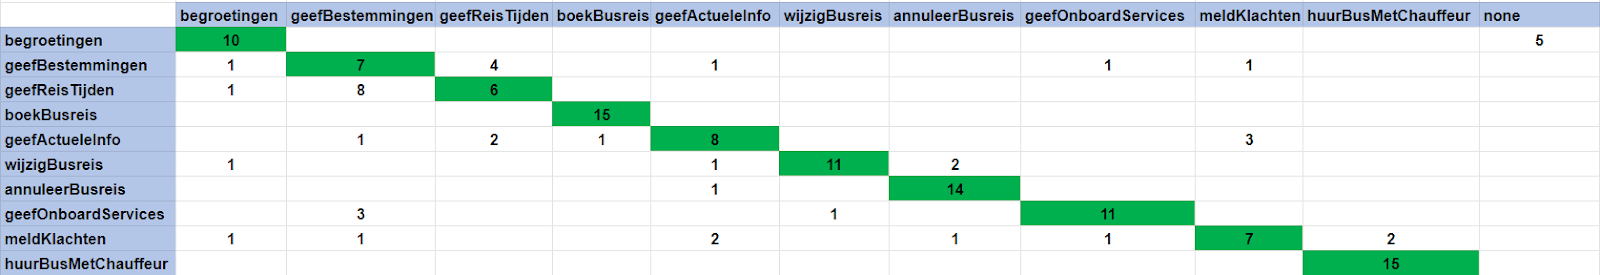
\includegraphics[width=\textwidth]{confusion-matrix-watson}
    \caption{Algemene confusion matrix intentherkenning zonder entities van IBM Watson}
\end{figure}

\begin{figure}[H]
    \label{fig:confusion-matrix-luis}
    \centering
    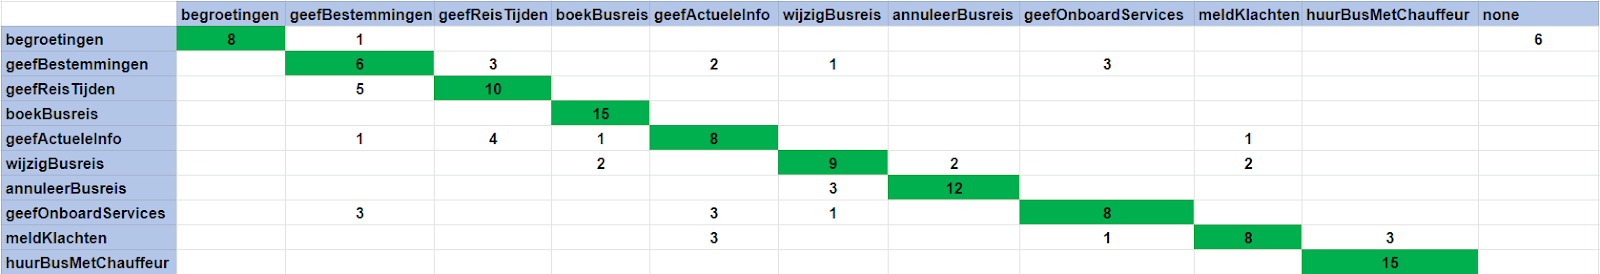
\includegraphics[width=\textwidth]{confusion-matrix-luis}
    \caption{Algemene confusion matrix intentherkenning zonder entities van LUIS}
\end{figure}

\begin{figure}[H]
    \label{fig:confusion-matrix-rasa}
    \centering
    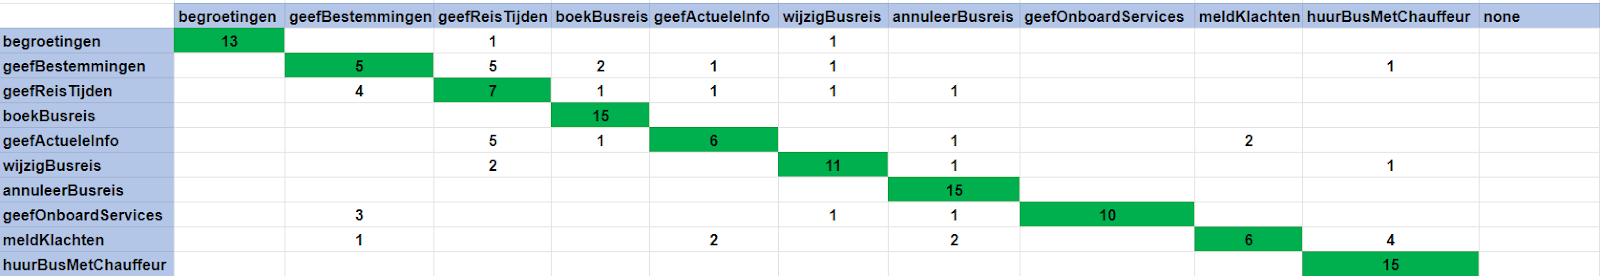
\includegraphics[width=\textwidth]{confusion-matrix-rasa}
    \caption{Algemene confusion matrix intentherkenning zonder entities van Rasa}
\end{figure}

\begin{figure}[H]
    \label{fig:confusion-matrix-wit}
    \centering
    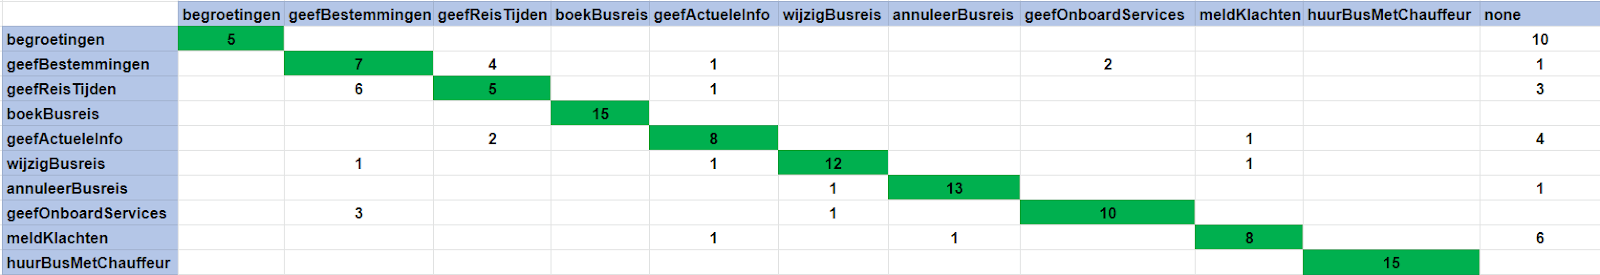
\includegraphics[width=\textwidth]{confusion-matrix-wit}
    \caption{Algemene confusion matrix intentherkenning zonder entities van Wit.ai}
\end{figure}

\begin{figure}[H]
    \label{fig:confusion-matrix-dialogflow}
    \centering
    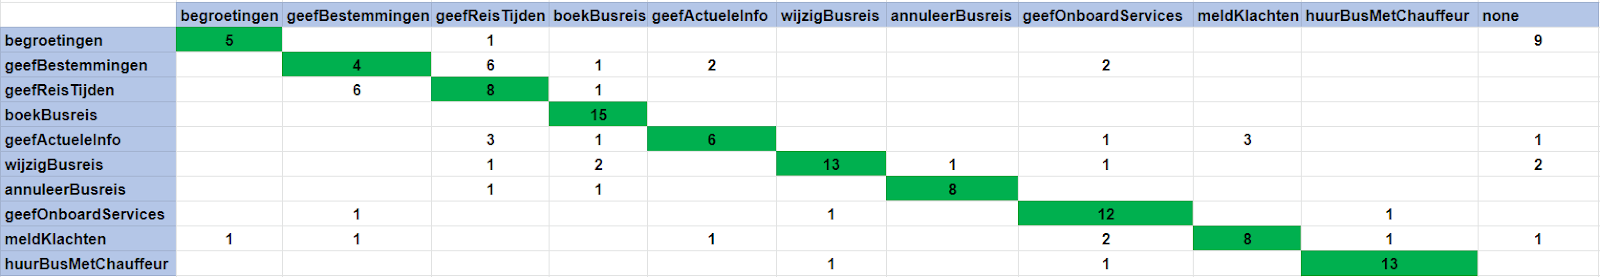
\includegraphics[width=\textwidth]{confusion-matrix-dialogflow}
    \caption{Algemene confusion matrix intentherkenning zonder entities van Dialogflow}
\end{figure}

\subsection{Onderlinge vergelijking}
\label{subsec:intent-onderling}

Op het eerste zicht valt het op dat er geen platform veel sterker presteert dan een andere. De gemiddelde resulaten van Wit.ai zijn de beste met eerstvolgende achtervolgers IBM Watson en Rasa. Die resultaten verschillen telkens maar 1 procent, dus dat is praktisch verwaarloosbaar. Dialogflow presteert wel duidelijk iets minder dan de andere 4 platformen. Daarnaast is het ook zichtbaar dat er ook duidelijke verschillen zitten in de gemiddelde resultaten van de cycli zelf. De resultaten van cyclus 2 liggen duidelijk hoger dan de andere gemiddelden en cyclus 5 scoort duidelijk het slechtst. Dat is volledig te wijten aan toeval van hoe het algoritme de dataset verdeeld heeft tijdens de uitvoering van cross validation. Als laatste is het ook belangrijk om stil te staan bij de f-scores van de individuele intents. Daarbij valt het op dat bepaalde intents opmerkelijk slecht scoren in vergelijking met andere. Dat komt doordat de platformen vaak die intents die slechter scoren met elkaar ging verwisselen. Dat kan ook duidelijk worden vastgesteld in de verschillende confusion matrices.

\begin{center}
    \begin{longtable}{| l | l | l | l | l |  l | l |}
        \hline
        \textbf{Platform} & \textbf{Cyclus 1} & \textbf{Cyclus 2} & \textbf{Cyclus 3} & \textbf{Cyclus 4} & \textbf{Cyclus 5} & \textbf{GEMIDDELD} \\ \hline
        \textbf{IBM Watson} & 0,70000 & 0,76667 & 0,67797 & 0,81356 & 0,56140 & \textbf{0,70508} \\ \hline  
        \textbf{LUIS} & 0,61017 & 0,76667 & 0,64407 & 0,76667 & 0,57143 & \textbf{0,67347} \\ \hline  
        \textbf{Rasa} & 0,66667 & 0,76667 & 0,66667 & 0,70000 & 0,63333 & \textbf{0,68667} \\ \hline  
        \textbf{Wit.ai} & 0,61818 & 0,67857 & 1,00000 & 0,67925 & 0,54902 & \textbf{0,71273} \\ \hline  
        \textbf{Dialogflow} & 0,64407 & 0,71429 & 0,67797 & 0,60714 & 0,56140 & \textbf{0,64111} \\ \hline  
        \textbf{GEMIDDELD} & \textbf{0,647818} & \textbf{0,738574} & \textbf{0,67797} & \textbf{0,60714} & \textbf{0,5614} &    \\ \hline
        \caption{Tabel met f-scores per platform voor intentherkenning zonder entities}                                    
    \end{longtable}
    \label{tbl:results-intent-no-entity}
\end{center}

\begin{figure}[H]
    \label{fig:chart-intent-no-entity}
    \centering
    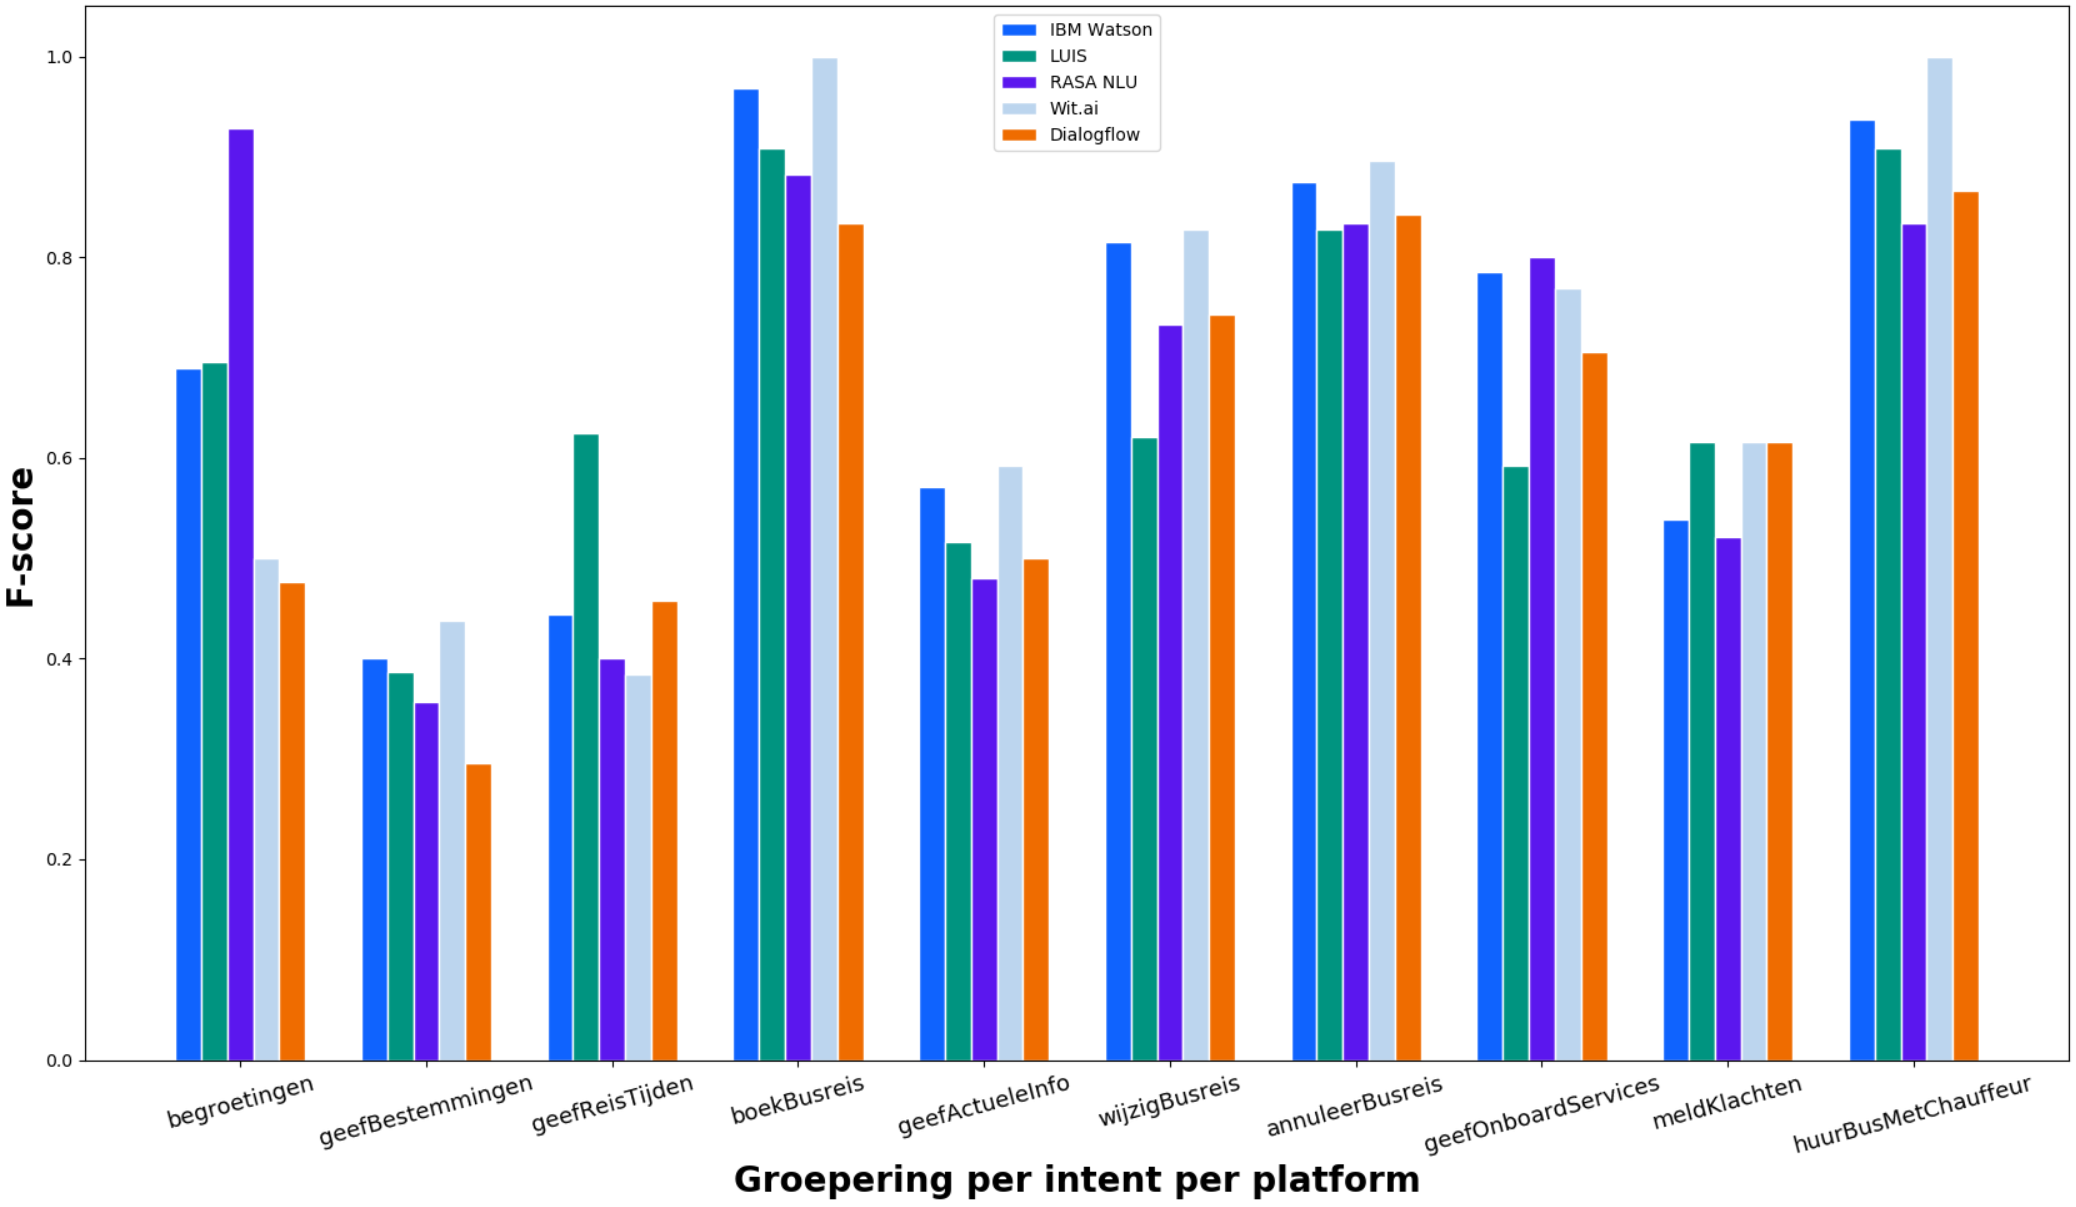
\includegraphics[width=\textwidth]{chart-intent}
    \caption{Grafiek die de f-scores per intent per platform visualiseert voor intentherkenning zonder entities}
\end{figure}

\section{Intent-en-entityherkenning}

Bij het tweede experiment, werd gekeken naar hoe goed de platformen entities kunnen afleiden uit de input en hoe het zit met intentherkenning bij het gebruik van entities. Daarbij werd in tegenstelling tot het eerste experiment maar 1 iteratie uitgevoerd, omdat het eerste experiment het hoofdexperiment is van deze bachelorproef en daar dus extra aandacht aan besteed werd. 5 fold cross validation uitvoeren neemt erg veel tijd in beslag, daarom dat er een keuze moest gemaakt worden. Voor dit experiment werd de dataset door middel van een algoritme verdeeld in 2 delen, een dataset om te trainen (80\% van de data) en een dataset om te valideren (20\% van de data). Alle platformen werden getraind en gevalideerd op een manier dat ze nu wel entities bevatten. Uit de resultaten valt het meteen op dat de f-scores gemiddeld hoger liggen dan bij het eerste experiment. Dit moet met een korrel zout genomen worden, doordat er maar 1 iteratie is uitgevoerd en omdat er nieuwe train-en-test datasets gegenereerd zijn. Door toeval kunnen er ‘makkelijkere’ testzinnen gebruikt zijn. Bij deze resultaten is het duidelijk dat IBM Watson de betere resultaten kan voorleggen en dat het in tegenstelling tot het vorige experiment Wit.ai is die het slechtst scoort.


\begin{center}
    \begin{longtable}{| l | l |}
        \hline
        \textbf{Platform} & \textbf{F-score} \\ \hline
        \textbf{IBM Watson} & 0,80000 \\ \hline  
        \textbf{LUIS} & 0,74576 \\ \hline  
        \textbf{Rasa} & 0,70000 \\ \hline  
        \textbf{Wit.ai} & 0,65455  \\ \hline  
        \textbf{Dialogflow} & 0,72414 \\ \hline  
        \caption{Tabel met f-scores per platform voor intentherkenning met het gebruik van entities}                                    
    \end{longtable}
    \label{tbl:results-intent-entity}
\end{center}

\subsection{Entityherkenning}

Het belangrijkste deel van dit experiment is het valideren van de entitiyherkenning. Daarbij werd gebruik gemaakt van zowel systeementiteiten als van zelf gedefinieerde entiteiten. IBM Watson heeft tot op heden geen systeementiteit die locaties kan herkennen in het Nederlands, dat kon dus niet beoordeeld worden. Bij LUIS is het nog een stuk erger, daar zijn er geen systeementiteiten in het Nederlands voor het herkennen van locaties, datums en tijdstippen. Dit bestond vroeger wel, maar dat is stopgezet in december 2018. Er is een alternatief die op basis van machine learning alles zou herkennen, maar dit bleek niet vlot te werken en dus geen resultaten op te leveren.

Door deze tekorten liggen de scores van beide platformen voor entityherkenning een stuk lager, maar op de andere entities scoren ze wel aanzienlijk goed. 

Uit de resultaten valt het meteen op dat Wit.ai de grote winnaar is bij het herkennen van parameterwaarden. Ook in de grafiek waarbij de scores per entity worden voorgesteld is het duidelijk. Wit.ai scoort op elke entiteit minstens even goed of een stuk beter dan zijn concurrenten.

\begin{center}
    \begin{longtable}{| l | l |}
        \hline
        \textbf{Platform} & \textbf{F-score} \\ \hline
        \textbf{IBM Watson} & 0,62687 \\ \hline  
        \textbf{LUIS} & 0,26923 \\ \hline  
        \textbf{Rasa} & 0,79452 \\ \hline  
        \textbf{Wit.ai} & 0,95556  \\ \hline  
        \textbf{Dialogflow} & 0,83544 \\ \hline  
        \caption{Tabel met f-scores per platform voor entityherkenning}                                    
    \end{longtable}
    \label{tbl:results-entity}
\end{center}

\begin{figure}[H]
    \label{fig:chart-entity}
    \centering
    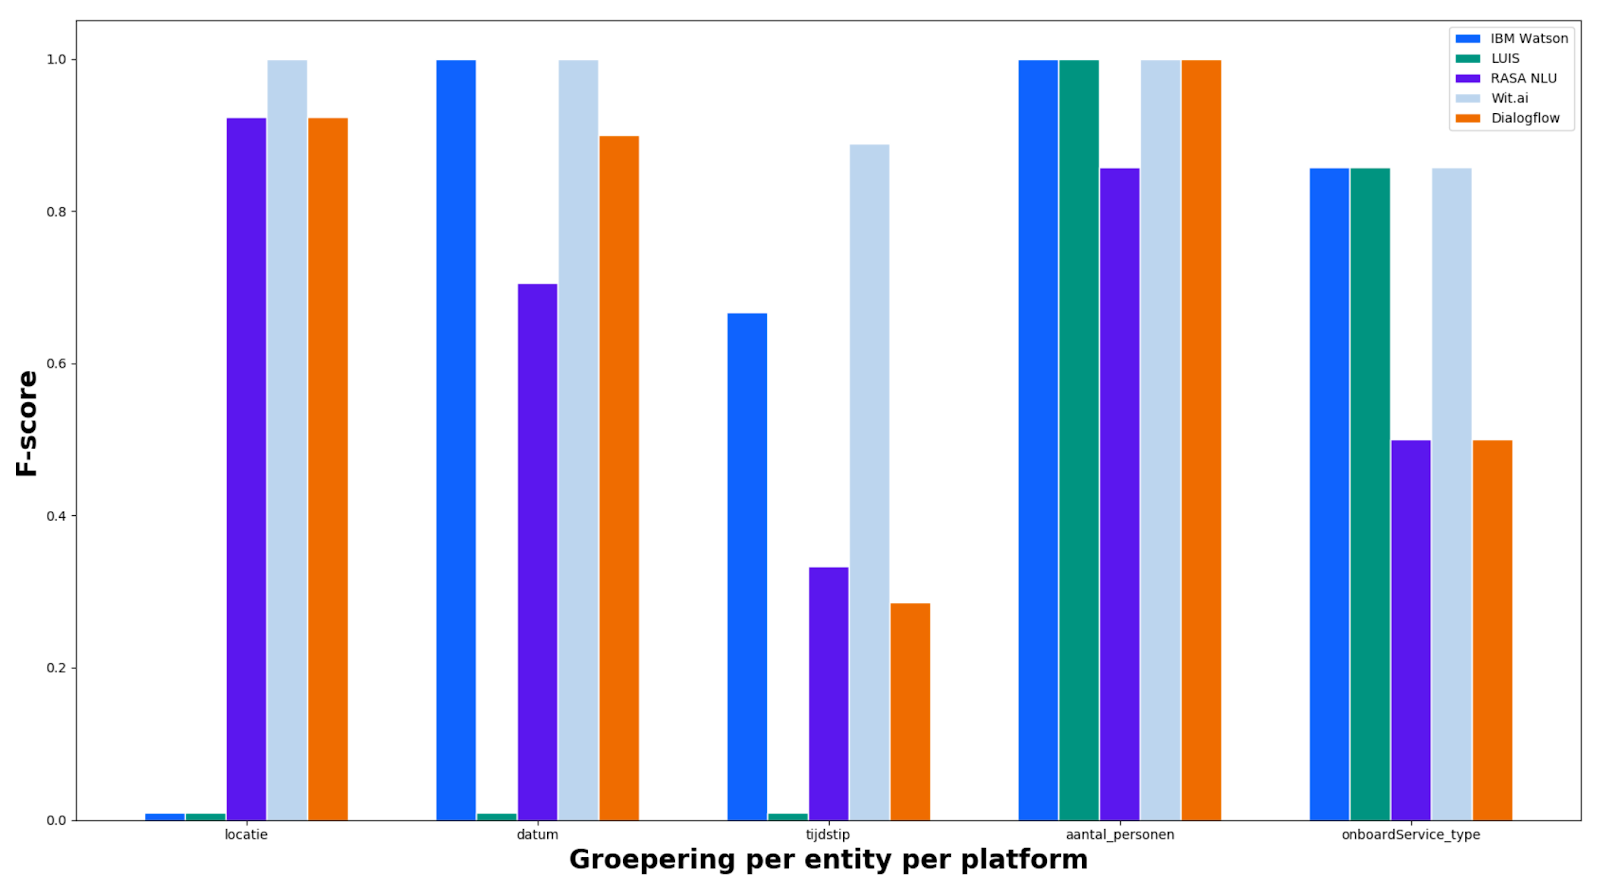
\includegraphics[width=\textwidth]{chart-entity}
    \caption{Grafiek die de f-scores per entity per platform visualiseert}
\end{figure}

\section{Invloed van spelling op Intent-en-entityherkenning}

Als laatste werd er gekeken naar hoe goed de platformen intents en entities kunnen herkennen als er een aanzienlijke hoeveelheid taalfouten in staan. Dit is delicaat om te valideren, omdat we met te kleine datasets werken om een volledig beeld te kunnen geven. Het is daarom ook slechts een indicatie van hoe goed de platformen hiermee omgaan. Er werden zowel taalfouten in intents als in entities beoordeeld. Opnieuw werd er slechts 1 iteratie uitgevoerd met dezelfde reden als voorgaand experiment. Er werd gebruik gemaakt van dezelfde datasets als bij het vorige experiment om een vergelijking te kunnen maken.

Wat opvalt is dat de resultaten van intentherkenning duidelijk lager liggen als er spellingsfouten gemaakt worden. Daarbij blijft IBM Watson wel het beste scoren. De sterkste daling in resultaten kunnen we vinden bij Dialogflow, die 22\% lager scoort.

\begin{center}
    \begin{longtable}{| l | l |}
        \hline
        \textbf{Platform} & \textbf{F-score} \\ \hline
        \textbf{IBM Watson} & 0,67797 \\ \hline  
        \textbf{LUIS} & 0,61017 \\ \hline  
        \textbf{Rasa} & 0,63333 \\ \hline  
        \textbf{Wit.ai} & 0,54545  \\ \hline  
        \textbf{Dialogflow} & 0,50000 \\ \hline  
        \caption{Tabel met f-scores per platform voor intentherkenning bij het gebruik van spellingsfouten}                                    
    \end{longtable}
    \label{tbl:results-intent-spelling}
\end{center}

\subsection{Entityherkenning}

Opnieuw werden ook de prestaties van entityherkenning in acht genomen. Daarbij gelden dezelfde limitaties als vorig experiment van IBM Watson en LUIS. Hierbij liggen de resultaten ook gemiddeld lager dan voordien. De grote winnaar blijft immers wel Wit.ai, die nog steeds heel erg goede resultaten kan voorleggen. De grootste dalers zijn Rasa en Dialogflow die respectievelijk dalen met 34\% en 27\%.

\begin{center}
    \begin{longtable}{| l | l |}
        \hline
        \textbf{Platform} & \textbf{F-score} \\ \hline
        \textbf{IBM Watson} & 0,56250 \\ \hline  
        \textbf{LUIS} & 0,20000 \\ \hline  
        \textbf{Rasa} & 0,44828 \\ \hline  
        \textbf{Wit.ai} & 0,81013  \\ \hline  
        \textbf{Dialogflow} & 0,57143 \\ \hline  
        \caption{Tabel met f-scores per platform voor entityherkenning bij spellingsfouten}                                    
    \end{longtable}
    \label{tbl:results-entity-spelling}
\end{center}

\begin{figure}[H]
    \label{fig:chart-entity-spelling}
    \centering
    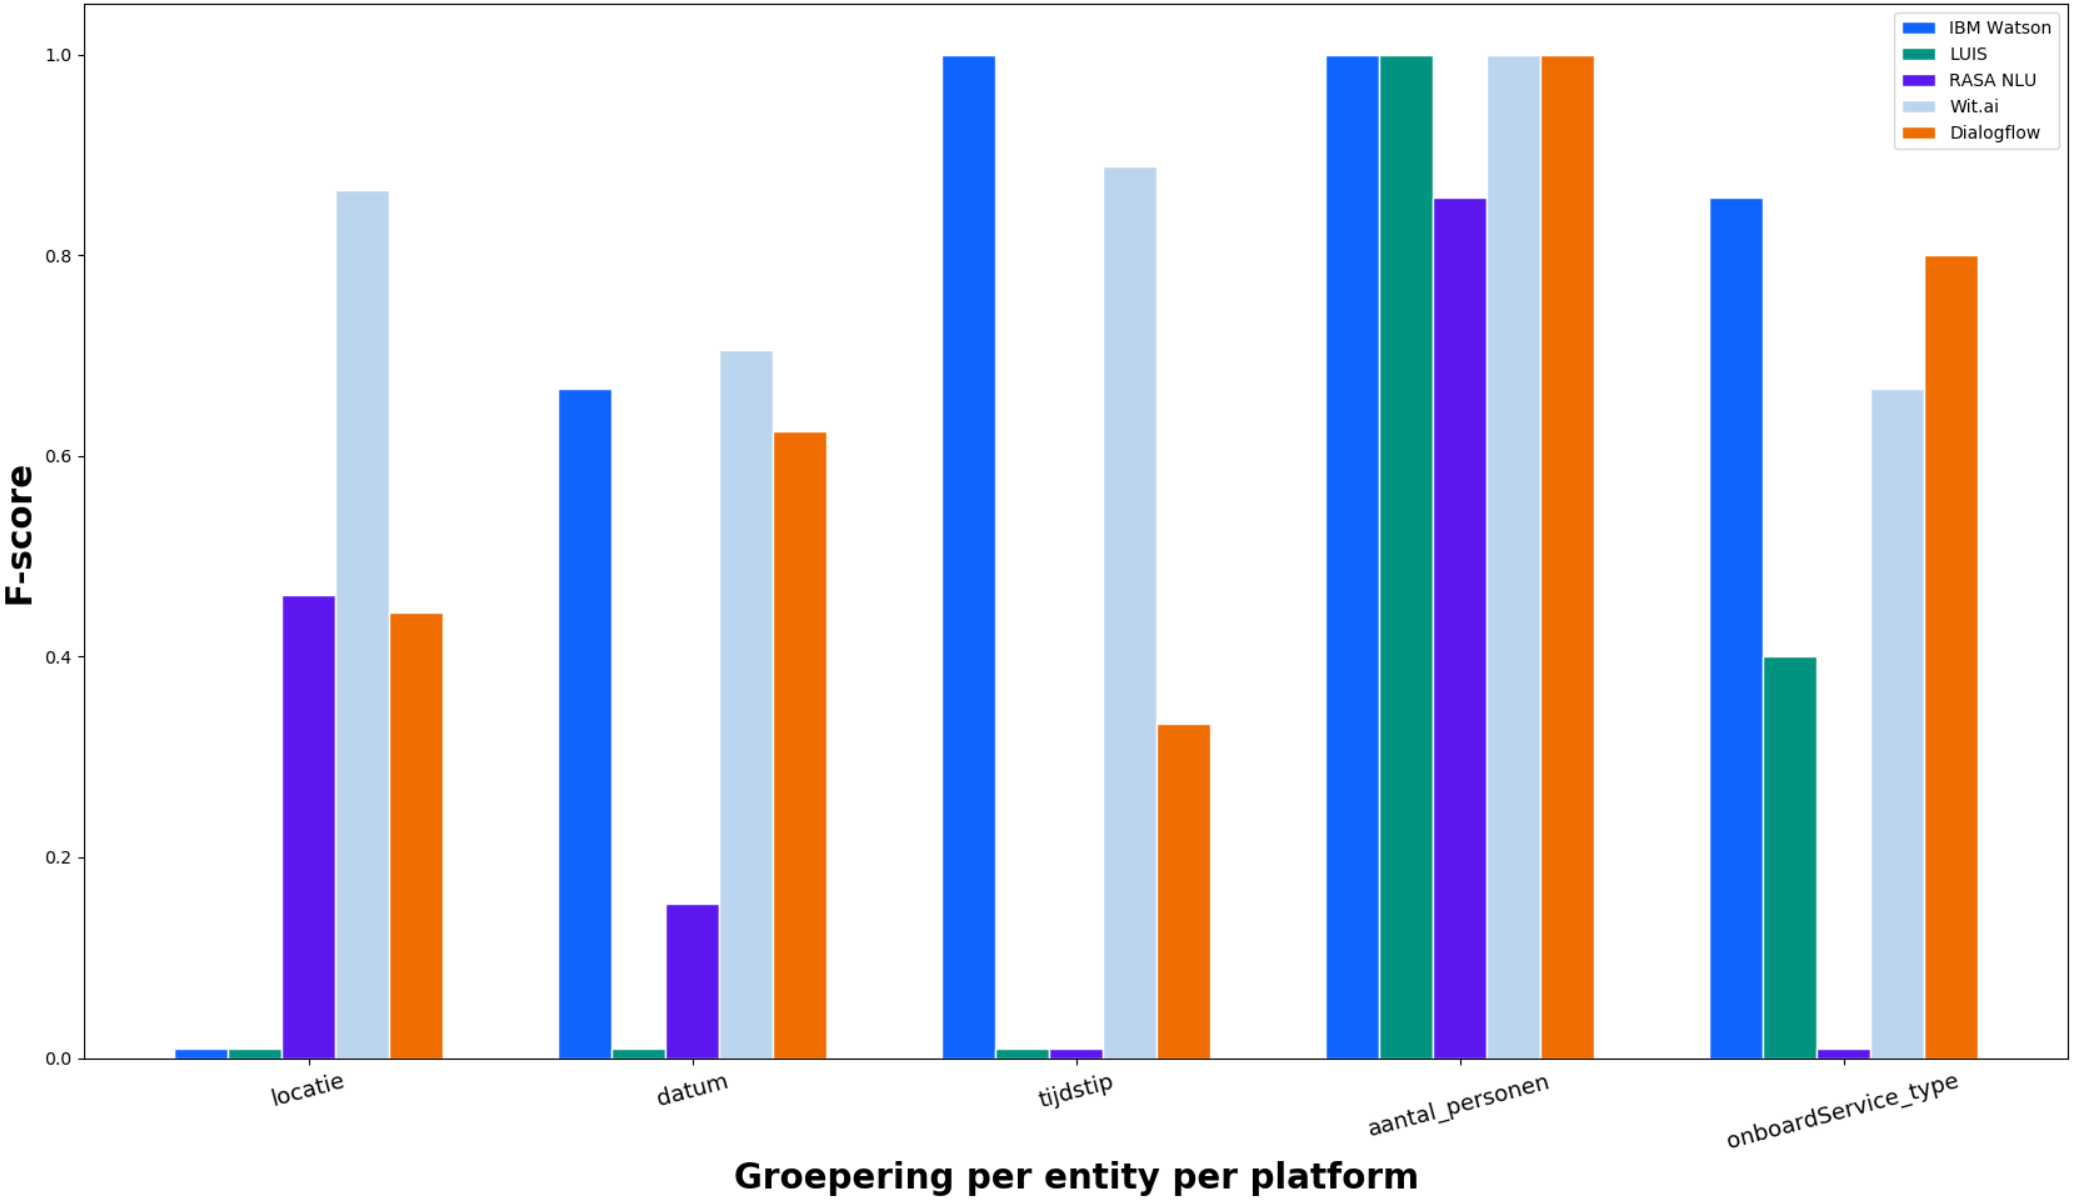
\includegraphics[width=\textwidth]{chart-entity-spelling}
    \caption{Grafiek die de f-scores per entity per platform visualiseert bij het gebruik van spellingsfouten}
\end{figure}















%%=============================================================================
%% Conclusie
%%=============================================================================

\chapter{Conclusie}
\label{ch:conclusie}

% Trek een duidelijke conclusie, in de vorm van een antwoord op de
% onderzoeksvra(a)g(en). Wat was jouw bijdrage aan het onderzoeksdomein en
% hoe biedt dit meerwaarde aan het vakgebied/doelgroep? 
% Reflecteer kritisch over het resultaat. In Engelse teksten wordt deze sectie
% ``Discussion'' genoemd. Had je deze uitkomst verwacht? Zijn er zaken die nog
% niet duidelijk zijn?
% Heeft het onderzoek geleid tot nieuwe vragen die uitnodigen tot verder 
%onderzoek?

Binnen deze bachelorproef is er een uitgebreid onderzoek gevoerd naar de verschillende gratis platformen die overweg kunnen met de Nederlandse taal om een chatbot te ontwikkelen, de meest interessante werden verder uitgediept. Er bestaat een grote verscheidenheid aan platformen en er is op dit moment niet veel informatie over de prestaties van deze platformen voor de Nederlandse taal. Digital product studio In The Pocket heeft regelmatig projecten waarbij het implementeren van een chatbot een meerwaarde kan bieden op het resultaat. Doordat In The Pocket
partner is van Google Cloud, werken ze vooral met de producten die aangeboden worden door Google. Het is voor hen een goede mogelijkheid om meer overzicht te krijgen in wat er op dit moment bestaat en hoe dit presteert voor het Nederlands. Daarbij werd er stilgestaan bij de verschillende functionaliteiten, de voor- en nadelen, de werking, de prestaties en de verschillende integratiemogelijkheden, zoals bijvoorbeeld met Slack of Facebook Messenger. De focus binnen deze bachelorproef lag op het vinden van het platform die het best verstaat wat de gebruiker juist bedoeld en ook belangrijke informatie zoals datums, locaties, tijdstippen, etc. kan extraheren. Daarbij werd ook rekening gehouden met spellingsfouten. De platformen zijn door middel van objectieve beoordelingstechnieken en verschillende experimenten getest.

Uit dit onderzoek kan geconcludeerd worden dat de resultaten van de verschillende platformen voor intentherkenning heel erg dicht bij elkaar liggen. Dit zorgt ervoor dat het moeilijk te besluiten is welk platform het beste presteert, aangezien dit op enkele procenten aankomt. Wit.ai kan de beste resultaten voorleggen met een verschil van minder dan één procent op IBM Watson. Wit.ai scoort wel slechter als er veel spellingsfouten in de voorbeeldzinnen staan. Daar zien we dat IBM Watson de duidelijke winnaar is en dat Wit.ai heel wat slechter scoort.

Op het vlak van entityherkenning is het wel duidelijk, Wit.ai steekt er bovenuit en geen enkel ander platform komt dicht in de buurt. Dialogflow presteert ook goed, maar niet goed genoeg om waardige concurrentie te zijn voor Wit.ai. Bij zowel het gebruik van spellingsfouten als zonder, is Wit.ai duidelijk de beste.

Wit.ai is vrij gemakkelijk te gebruiken en heeft als grote voordelen dat het volledig gratis te gebruiken is en dat het bijna alle talen ondersteunt. De documentatie voor zowel de grafische interface als de API is ook goed uitgewerkt. De API werkt wel niet optimaal. Het is een aantal keer voorgevallen dat niet alle data die werd verstuurd, ook effectief in het platform terecht kwam, terwijl de API wel een bericht terug stuurde dat alles succesvol was toegevoegd. Het duurde vaak lang tot de applicatie getraind was, dit kan problemen veroorzaken bij applicaties die groter zijn en meer data bevatten.

Dialogflow heeft de beste integratiemogelijkheden. Bij Wit.ai zijn deze beperkt, doordat het deel uitmaakt van Facebook. Het is natuurlijk wel altijd mogelijk om zelf een applicatie op te zetten door gebruik te maken van de API’s en SDK’s.

Alhoewel dat er objectieve beoordelingstechnieken gebruikt zijn, geeft dit onderzoek enkel een indicatie van welk platform het beste presteert. Er is een fictieve dataset opgesteld waarin een aantal voorbeeldzinnen werden toegevoegd die gebruikt werden. Deze dataset is te klein om een sluitend antwoord te formuleren over welk platform de beste is. Een representatieve dataset opstellen was in dit onderzoek niet mogelijk doordat er een beperkte tijd is. Er is ook beperkt tot de (grotendeels) gratis platformen, wat dus niet kan uitsluiten dat er bepaalde betalende platformen beter presteren. Dit onderzoek is ook volledig op Nederlandse data uitgevoerd, maar sommige platformen staan daarbij nog niet zo ver als waar ze staan bij de Engelse taal.

Dit onderzoek biedt een mooi startpunt voor verder onderzoek, waarin er gebruik gemaakt kan worden van representatieve datasets om te beoordelen of er daar andere conclusies worden bekomen. Het is ook interessant om te onderzoeken of dat er grote verschillen zijn in resultaten als er Engelse data gebruikt wordt. Daarnaast is het ook een mooi startpunt om dit onderzoek verder uit te breiden met betalende platformen om de verschillen vast te leggen.




%%=============================================================================
%% Bijlagen
%%=============================================================================

\appendix
\renewcommand{\chaptername}{Appendix}

%%---------- Onderzoeksvoorstel -----------------------------------------------

\chapter{Onderzoeksvoorstel}

Het onderwerp van deze bachelorproef is gebaseerd op een onderzoeksvoorstel dat vooraf werd beoordeeld door de promotor. Dat voorstel is opgenomen in deze bijlage.

% Verwijzing naar het bestand met de inhoud van het onderzoeksvoorstel
%---------- Inleiding ---------------------------------------------------------

\section{Introductie} % The \section*{} command stops section numbering
\label{sec:introductie}
Natural Language Processing (NLP) is een term die voor velen onbekend in de oren klinkt, maar toch is het iets waar de meeste mensen dagelijks mee in contact komen. Denk maar aan een zoekmachine op het internet, virtuele assistenten en chatbots. NLP betekent de mogelijkheid om als machine menselijke taal te begrijpen en te verwerken. Tijdens deze bachelorproef zal de focus liggen op de chatbots. Chatbots zijn niet meer weg te denken uit onze maatschappij, ze hebben al meermaals aangetoond dat ze nuttig zijn bij het ondersteunen van menselijke taken en dat ze een aanzienlijke hoeveelheid werk kunnen vergemakkelijken \autocite{Atwell2007}.  De impact ervan is de voorbije jaren alleen maar gestegen en deze trend zal ook niet meteen ophouden \autocite{BRAIN2019}. Chatbots vinden vooral hun intrede bij de klantenservice van bedrijven, maar ook bij het bestellen van producten, weersvoorspellingen, advies, nieuws, enz. Er zijn tientallen tools en ontwikkelmethoden op de markt die het ontwikkelen van chatbots mogelijk maken. Bedrijven zoals Google, Facebook, Amazon, IBM en Microsoft hebben elk hun eigen NLP-platform ontwikkeld om het creëren van chatbots voor andere bedrijven eenvoudiger te maken. Elk van deze platformen hebben hun eigen sterktes en tekortkomingen en worden continu bijgewerkt en verbeterd. Een digital product studio als In The Pocket heeft regelmatig projecten lopen met klanten waarbij het implementeren van een chatbot een toegevoerde waarde kan betekenen voor het eindresultaat. In The Pocket is officiële partner van Google Cloud en gebruikt dus voornamelijk hun producten. Het is daarom interessant voor hen om te onderzoeken hoe de verschillende cloud platformen momenteel van elkaar verschillen en waar bepaalde frameworks meer in uitblinken dan andere. Dit onderzoek kan voor hen een goed uitgangspunt zijn om in de toekomst te bepalen welk NLP-platform de beste oplossing biedt voor een bepaald project. Deze onderzoeksdoelstelling kan worden opgedeeld in een aantal specifieke deelvragen:

\begin{itemize}
  \item Met welk platform kun je de meest kwalitatieve chatbot bouwen op een bepaald criteria ? 
  \item Wat zijn de verschillende voordelen en tekortkomingen van bepaalde platformen en welke prijs is daar aan verbonden ?
  \item Welke tool reageert het best op user input en hoe gaat het om met taalvariaties en emoties ?
  \item Welk platform biedt de beste compatibiliteit en integraties aan ?
\end{itemize}

%---------- Stand van zaken ---------------------------------------------------

\section{State-of-the-art}
\label{sec:state-of-the-art}
Er is al veel onderzoek gedaan naar artificiële intelligentie en machineleertechnieken, maar omdat alles zo snel evolueert, is het belangrijk dat we onderzoeken blijven voeren en steeds op zoek blijven  gaan naar meer antwoorden op de problemen die zich nog stellen. Volgens  \textcite{Hussain2019} zijn er nog veel verbeterpunten mogelijk op het vlak van chatbots. Zo zou er meer focus moeten liggen op het beter verstaan van taalkundige elementen door bijvoorbeeld emotionele-en sentimentsanalyses uit te voeren en er zou ook een betere standaard moeten zijn om de kwaliteit van chatbots te testen. Een eerder onderzoek heeft aangetoond dat mensen anders communiceren als ze weten dat ze met een machine converseren. Zo zouden mensen hun taal aanpassen als ze tegen een chatbot praten, zoals mensen ook doen als ze tegen een kind bezig zijn \autocite{Hill2015}.
We kunnen concluderen dat chatbots een duidelijke meerwaarde hebben binnen onze maatschappij en dat onderzoek rond chatbots nog kan blijven verbeteren, maar hoe zit het met de onderlinge vergelijking tussen verschillende chatbots ? Zijn bepaalde chatbots beter dan andere ? Volgens het onderzoek van \textcite{Russis2018} is de tool die IBM (Watson) aanbiedt om chatbots in de cloud te bouwen de beste op de markt met als dichte achtervolgers Microsoft (LUIS) en Google (Dialogflow). Dit wordt betwist door het onderzoek van \textcite{Langen2017}, want zij besluiten dat LUIS (Microsoft) veruit het beste platform is. In 2019 is er echter veel veranderd in de wereld van NLP. Dat komt door de modellen die gebaseerd zijn op de transformers. Een voorbeeld van zo’n model is BERT, die ontwikkeld is door Google. Het concept van een transformer zorgt er voor dat relaties tussen woorden in zinnen beter kunnen gevonden worden door machines \autocite{Joshi2019}. Chatbotplatformen gebruiken deze modellen om betere resultaten op te leveren. Een voorbeeld hiervan is Reply.ai, die BERT sterk gebruikt. Doordat transformers zo’n grote intrede gemaakt hebben, zijn vele voorgaande studies over welk platform de voorkeur krijgt geneutraliseerd. Een vergelijkende studie anno 2020 is dan ook zeker interessant om terug een beter overzicht van de actualiteit te krijgen.


% Voor literatuurverwijzingen zijn er twee belangrijke commando's:
% \autocite{KEY} => (Auteur, jaartal) Gebruik dit als de naam van de auteur
%   geen onderdeel is van de zin.
% \textcite{KEY} => Auteur (jaartal)  Gebruik dit als de auteursnaam wel een
%   functie heeft in de zin (bv. ``Uit onderzoek door Doll & Hill (1954) bleek
%   ...'')
%---------- Methodologie ------------------------------------------------------
\section{Methodologie}
\label{sec:methodologie}

Bij het uitwerken van deze bachelorproef kan het volledige proces worden opgedeeld in 5 fases.
In de eerste fase zal er algemene uitleg rond chatbots plaatsvinden en zullen belangrijke begrippen toegelicht worden. Er zal ook stilgestaan worden bij de uitdagingen en tekortkomingen van chatbots op dit moment. Tijdens de tweede fase zal er een vergelijkende studie worden uitgevoerd, waarbij er een aantal NLP-platformen zullen worden vergeleken met elkaar. Ze zullen worden vergeleken op vaste criteria zoals prijs, integratiemogelijkheden, complexiteit, ontwikkeltijd, ondersteuning voor verschillende (programmeer) talen, pre-built entities/intents, spraakherkenning, ... De belangrijkste voor-en nadelen zullen ook uitvoerig besproken worden. Er zal hier niet alleen naar de grote marktspelers worden gekeken, maar ook naar kleinere platformen die minder in de belangstelling staan zoals Recast.ai, ChatFuel, RASA, AgentBot, Botsify, reply.ai, … Tijdens de derde fase zullen de drie meest interessante platformen uit deze lijst geselecteerd worden en zal er een testscenario worden opgesteld waarbij er een aantal factoren van deze 3 gekozen tools uitvoerig getest en geëvalueerd zullen worden. Voor het testscenario zal er een dataset voorzien worden met testdata waarmee elk gekozen platform zal getraind worden. Daarna zullen de chatbots beoordeeld worden op de verschillende criteria door middel van conversaties waarbij er zal worden gekeken naar de volgende criteria:\bigskip

\begin{itemize}
    \item Hoe reageert de chatbot op een normale eenvoudige conversatie met weinig moeilijke zinnen ?
    \item Hoe gaat de chatbot om met negatieve expressies ? Dit kunnen klantenklachten zijn of negatieve emoties.
    \item Hoe goed neemt de chatbot slecht gevormde zinnen en woorden op en hoe accuraat is het antwoord ?
    \item Hoe accuraat blijft het antwoord van de chatbot als hij erg complexe zinstructuren moet verwerken ? Dit kunnen zinnen zijn die heel erg lang zijn, veel moeilijke woorden en werkwoorden bevatten, vragen en bevelen op het zelfde moment bevatten, quote's bevatten, ...
    \item Hoe goed gaat de chatbot om met berichten die niets hebben te maken met de scenario’s waarvoor hij is getraind ?
    \item Hoe goed herkent de chatbot het verschil tussen een vraag en een bevel ?
\end{itemize}

\bigskip
Tijdens de volgende fase van het proces zullen de chatbots die gebouwd zijn met de top drie platformen het testscenario doorlopen en zullen alle resultaten geanalyseerd worden.
De vijfde en laatste fase zal dienen voor de uiteindelijke vergelijking van alle resultaten die werden bekomen met de vorige fasen en zal er een conclusie gevormd worden.


%---------- Verwachte resultaten ----------------------------------------------
\section{Verwachte resultaten}
\label{sec:verwachte_resultaten} 

Een verwachting is dat er geen concrete voorkeur zal zijn voor een platform in verband met simpele conversaties met korte en duidelijke zinnen. Als het aankomt op nieuwe trainingsdata, dan is de verwachting dat LUIS het beste zal presteren door de active learning technologie die er in geïmplementeerd is. DialogFlow zou volgens eerder onderzoek dan weer het beste presteren op het herkennen van berichten die niets te maken hebben met waarvoor de chatbot is getraind \autocite{Russis2018}. Op accuraatheid zou Reply.ai de beste resultaten moeten kunnen voorleggen door het sterk gebruik van BERT. Daarentegen wordt er verwacht dat de integratiemogelijkheden van LUIS, Watson en DialogFlow hoger scoren dan van de andere concurrenten, omdat dit de grotere marktspelers zijn op vlak van chatbotplatformen.

%---------- Verwachte conclusies ----------------------------------------------
\section{Verwachte conclusies}
\label{sec:verwachte_conclusies}

Uit dit onderzoek verwachten we te kunnen concluderen dat het wel degelijk interessant is voor In The Pocket om in bepaalde scenario’s over te stappen naar een alternatief in plaats van Google producten. Indien er een beperkt budget is, dan verwachten we dat het nog steeds mogelijk is om door te werken met Dialogflow of Wit.ai, omdat deze gratis zijn. Op het moment dat de complexiteit toeneemt en de accuraatheid prioriteit wordt, dan wordt er verwacht dat het beter is om over te stappen naar LUIS (Microsoft) of Reply.ai. Bij de keuze naar een platform met veel integratiemogelijkheden zou de voorkeur uitgaan naar DialogFlow, LUIS of Watson, maar opnieuw zal het budget daar een belangrijke factor in zijn.



%%---------- Andere bijlagen --------------------------------------------------
% TODO: Voeg hier eventuele andere bijlagen toe
%\input{...}

%%---------- Referentielijst --------------------------------------------------

\printbibliography[heading=bibintoc]

\end{document}
